%4619055 課題3 パルス回路
\documentclass[12pt]{jarticle}
\usepackage{TUSIreport}
\usepackage{otf}
\usepackage{graphicx}
\usepackage{amsmath}
\usepackage{amssymb}
\usepackage{hhline}
\usepackage{fancybox,ascmac}
\usepackage{url}
%%%%%%%%%%%%%%%%%%
\begin{document}
%%%%%%%%%%%%%%%%%%%%%%%%%%%%%%%%%%%%%%%%%%%%%%%%%%%%%%%%
% 表紙を出力する場合は,\提出者と\共同実験者をいれる
% \提出者{科目名}{課題名}{提出年}{提出月}{提出日}{学籍番号}{氏名}
% \共同実験者{一人目}{二人目}{..}{..}{..}{..}{..}{八人目}
%%%%%%%%%%%%%%%%%%%%%%%%%%%%%%%%%%%%%%%%%%%%%%%%%%%%%%%
\提出者{情報工学実験1}{課題3 パルス回路}
{2020}{6}{22}{4619055}{辰川力駆}

\共同実験者{}{}{}{}{}{}{}{}
\追加実験者{}{}
\表紙出力

\section{実験の要旨}
本実験では、トランジスタパルス回路を中心に「微分回路」、
「パルス増幅回路」、「スイッチング回路」、「無安定マルチバイブレータ」、
「双安定マルチバイブレータ」についてパルス技術の基礎となっている概念について検討を行う。

\section{実験の目的}
パルス回路の動作、原理、特性を実験により理解し、パルス技術の基礎を習得する。

\section{実験装置・実験方法}
パルス回路実験装置(PED-101A)、オシロスコープ、ファンクションジェネレータ\\

実験装置には直流電流が組み込まれている。
100(V)電源を接続後、スイッチをONにすることで電源が供給される。
また、回路定数はセレクタピンで選択できる。

\subsection{微分回路}
\begin{enumerate}
    \item 実験回路を図\ref{fig1}に示す。
          $R = 20k\Omega$、$C = 0.01\mu F$として、
          入力端子(左側)にファンクションジェネレータを接続し、短形波を入力する。
          ただし、短形波の周波数は約$1kHz$、振幅は$5\sim6(V)$とする。
          このときの入出力波形をオシロスコープで観測する。
    \item $C$と$R$の値を変えて同様のことを行う(全4種類)。
\end{enumerate}
\subsection{積分回路}
\begin{enumerate}
    \item 実験回路図を図\ref{fig2}に示す。
    \item 微分回路と同様の測定を行う。
\end{enumerate}
\subsection{スイッチング回路}
\begin{enumerate}
    \item 図\ref{fig3}の回路中の抵抗値を
          $R_g = 40k\Omega$、$R_c = 1k\Omega$とし、
          入力端子に短形波(周波数$20kHz$、振幅$5\sim6$($V$))を入力し、
          出力波形の立ち下がり時間を測定する
          (このとき$R_g$と並列に繋がっているスピードアップコンデンサは外しておく)。
    \item $R_g$、$R_c$の値を変えて同様のことを行う(2、3種類程度)
    \item スピードアップコンデンサを$R_g$と並列に挿入した場合について1.と同様の測定を行う。
\end{enumerate}

\clearpage

\begin{figure}[h]
    \begin{minipage}{0.5\hsize}
        \begin{center}
            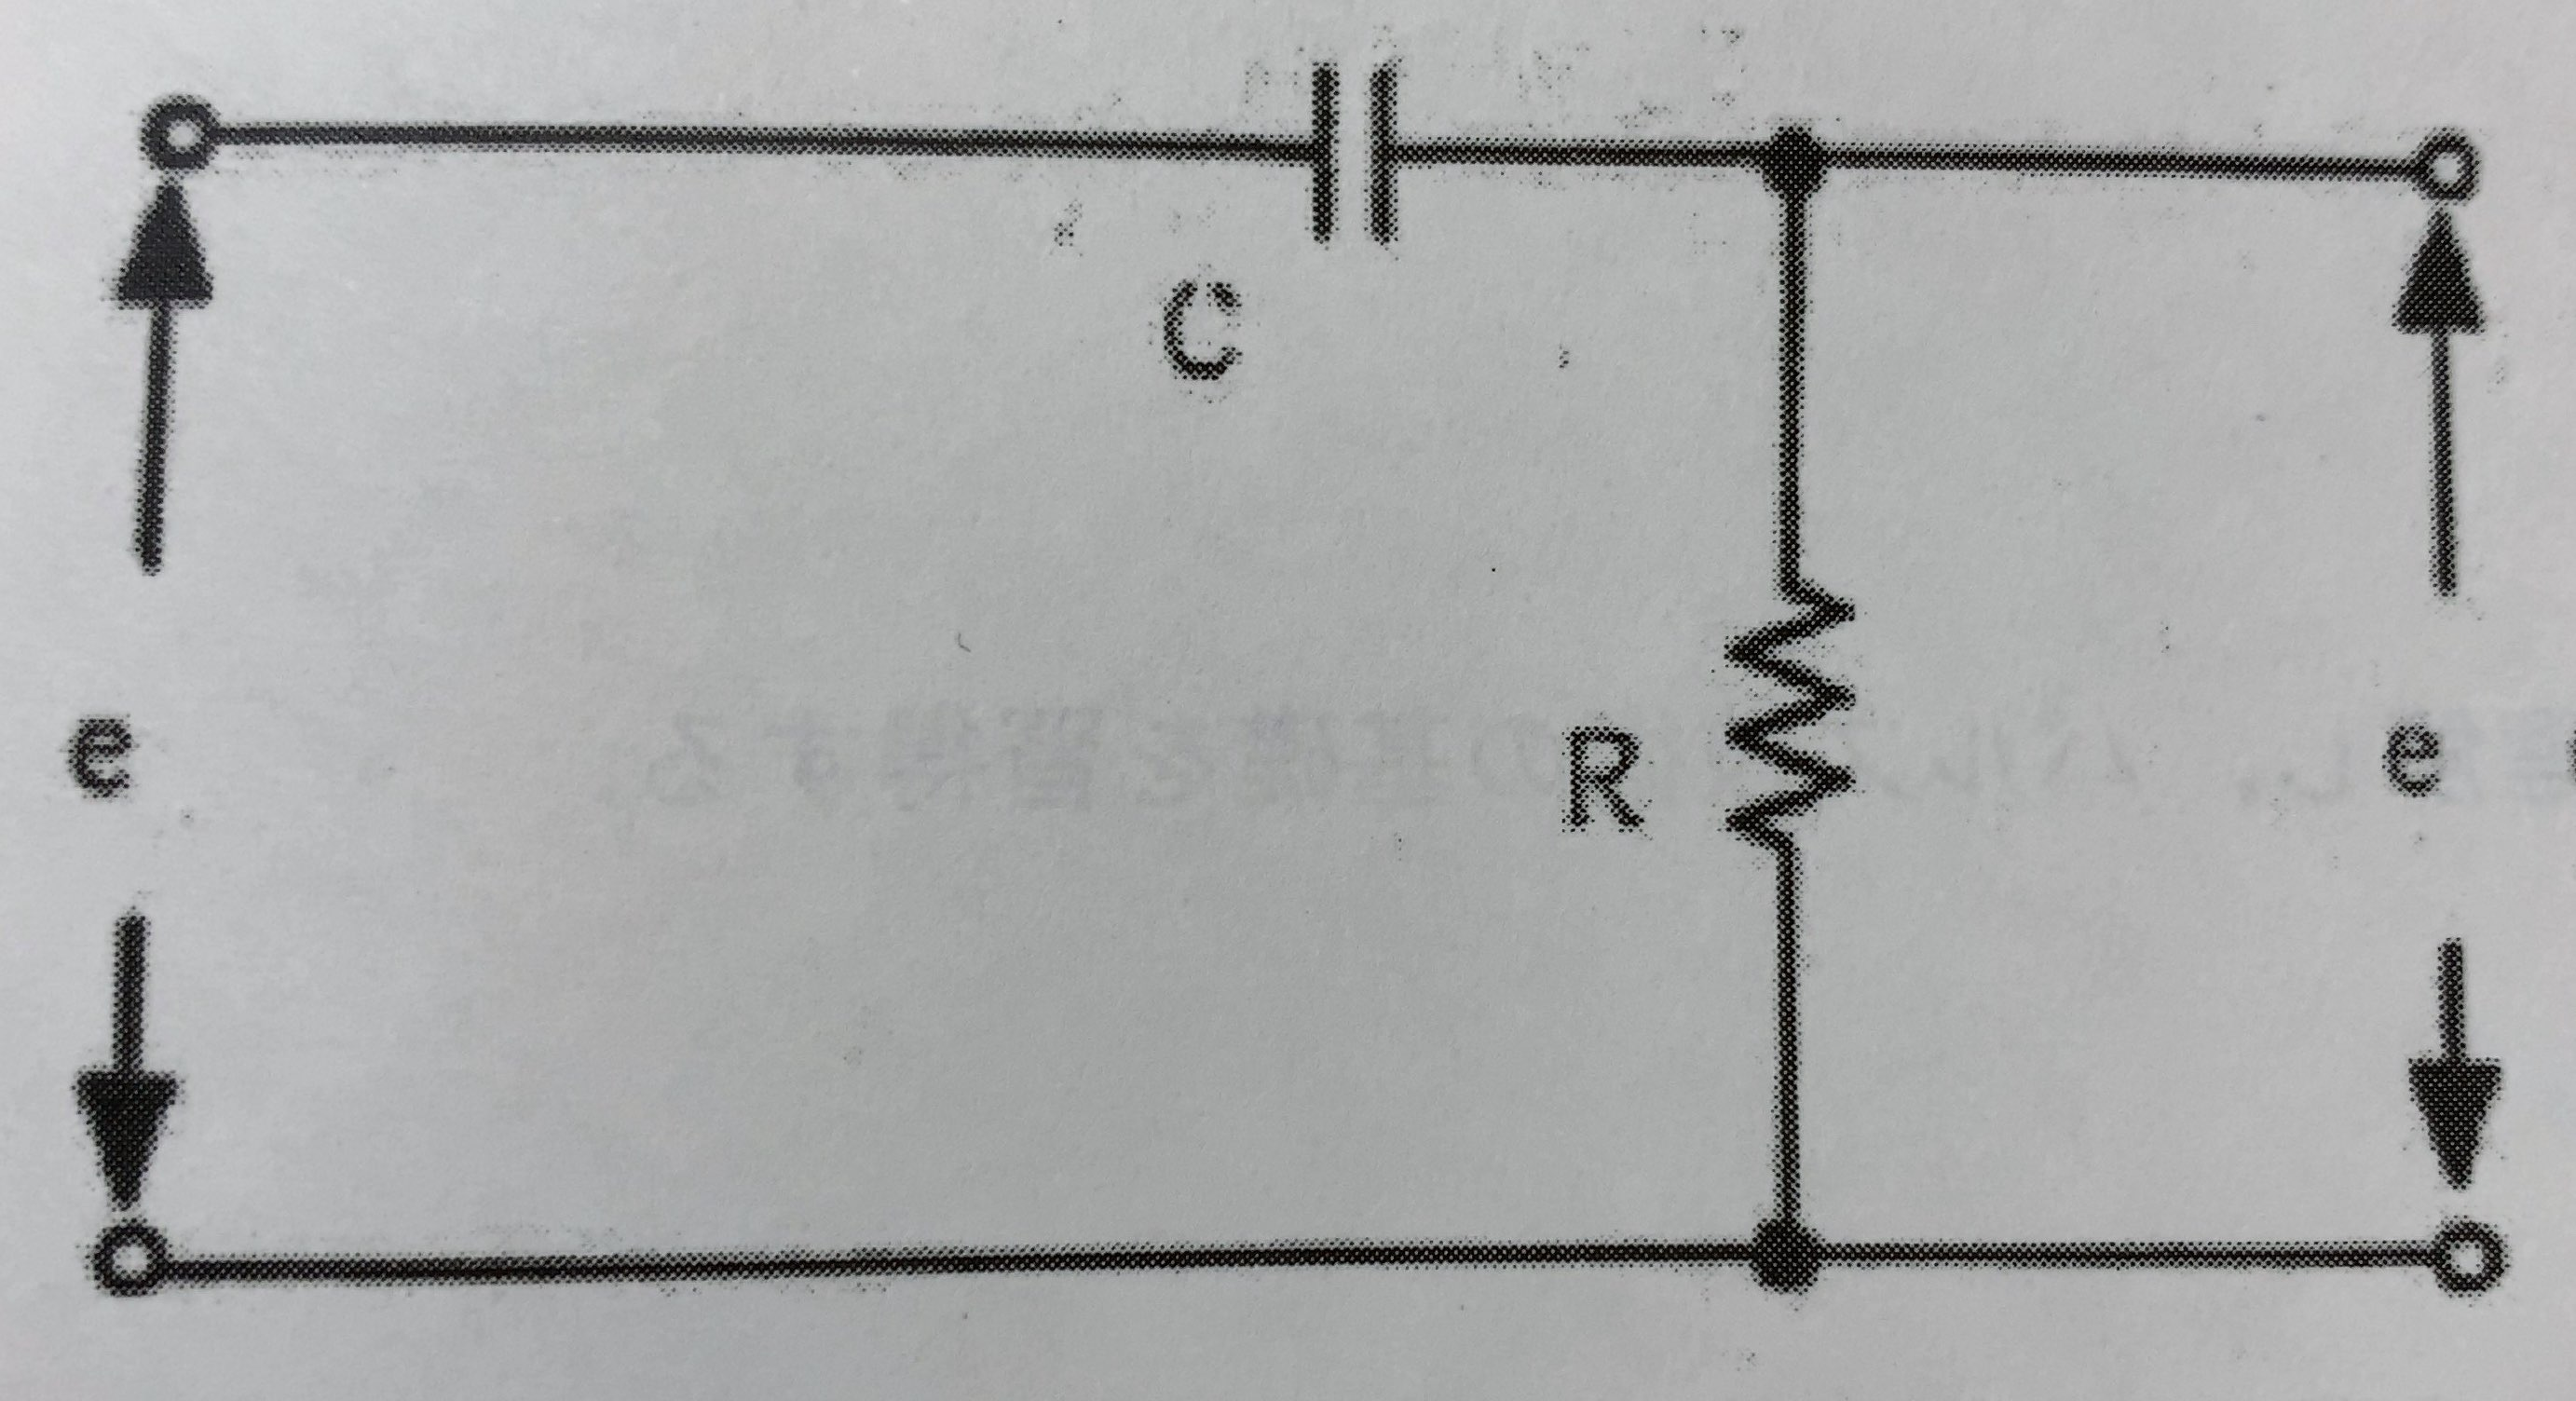
\includegraphics[bb=0 0 2765 1504,height=4cm]{parusu_1.jpg}
        \end{center}
        \caption{微分回路}
        \label{fig1}
    \end{minipage}
    \begin{minipage}{0.5\hsize}
        \begin{center}
            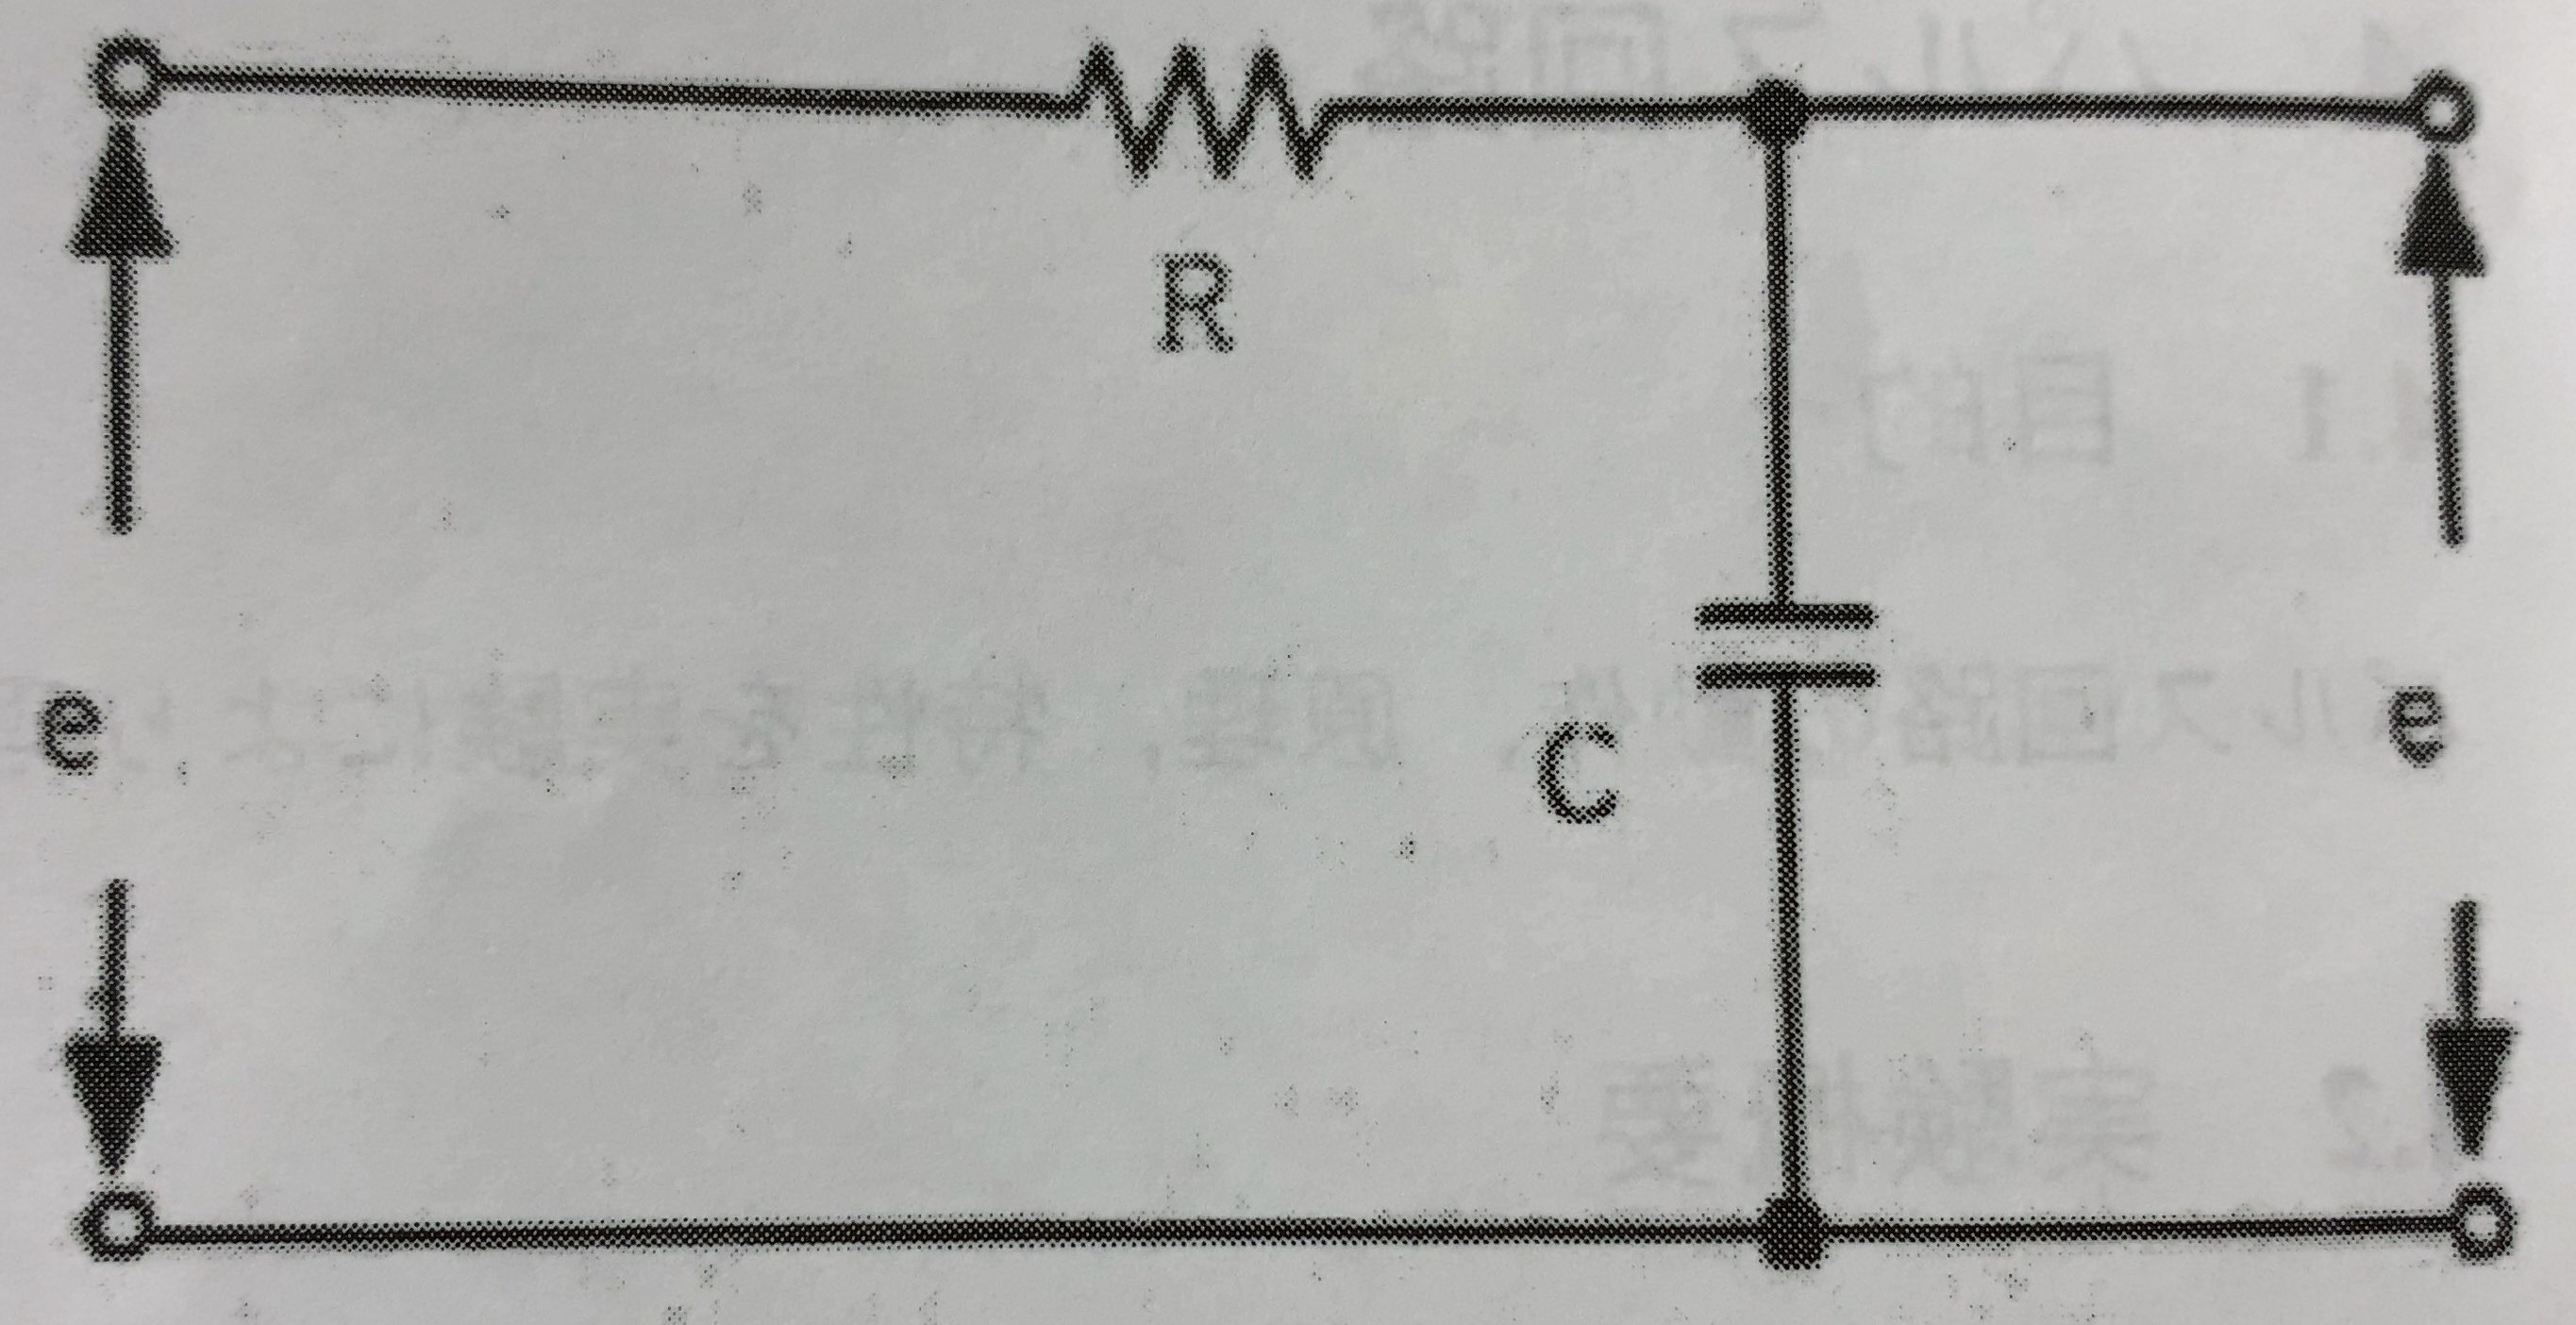
\includegraphics[bb= 0 0 2730 1404,height=4cm]{parusu_2.jpg}
        \end{center}
        \caption{積分回路}
        \label{fig2}
    \end{minipage}
\end{figure}

\subsection{パルス増幅回路}
\begin{enumerate}
    \item 図\ref{fig4}の回路中の抵抗値を
          $R_g = 500\Omega$、$R_c = 5k\Omega$、$R_e = 0\Omega$とし、
          入力端子に振幅$1(V)$程度の正弦波を入力する。
          次に正弦波に周波数を$100\sim100kHz$まで変化させ、
          増幅率を求める。ただし、増幅率$G$は次式
          \begin{equation}
              G = \frac{V_{out}}{V_{in}}
          \end{equation}
          で与えられる。
          測定は、$10\sim15$種類の周波数に対して行えばよいが、対数的に変化させること。
    \item$R_g$を$1k\Omega$にして1.と同様の測定を行う。
    \item$R_c = 1k\Omega,R_g = 500\Omega$に設定し、
          $R_e=0\Omega、100\Omega$としたときの周波数特性を
          それぞれ測定する(増減率$G$を求めよという意味)。
          ただし、入力信号の条件は1.と同様でよい。
\end{enumerate}

\begin{figure}[h]
    \begin{center}
        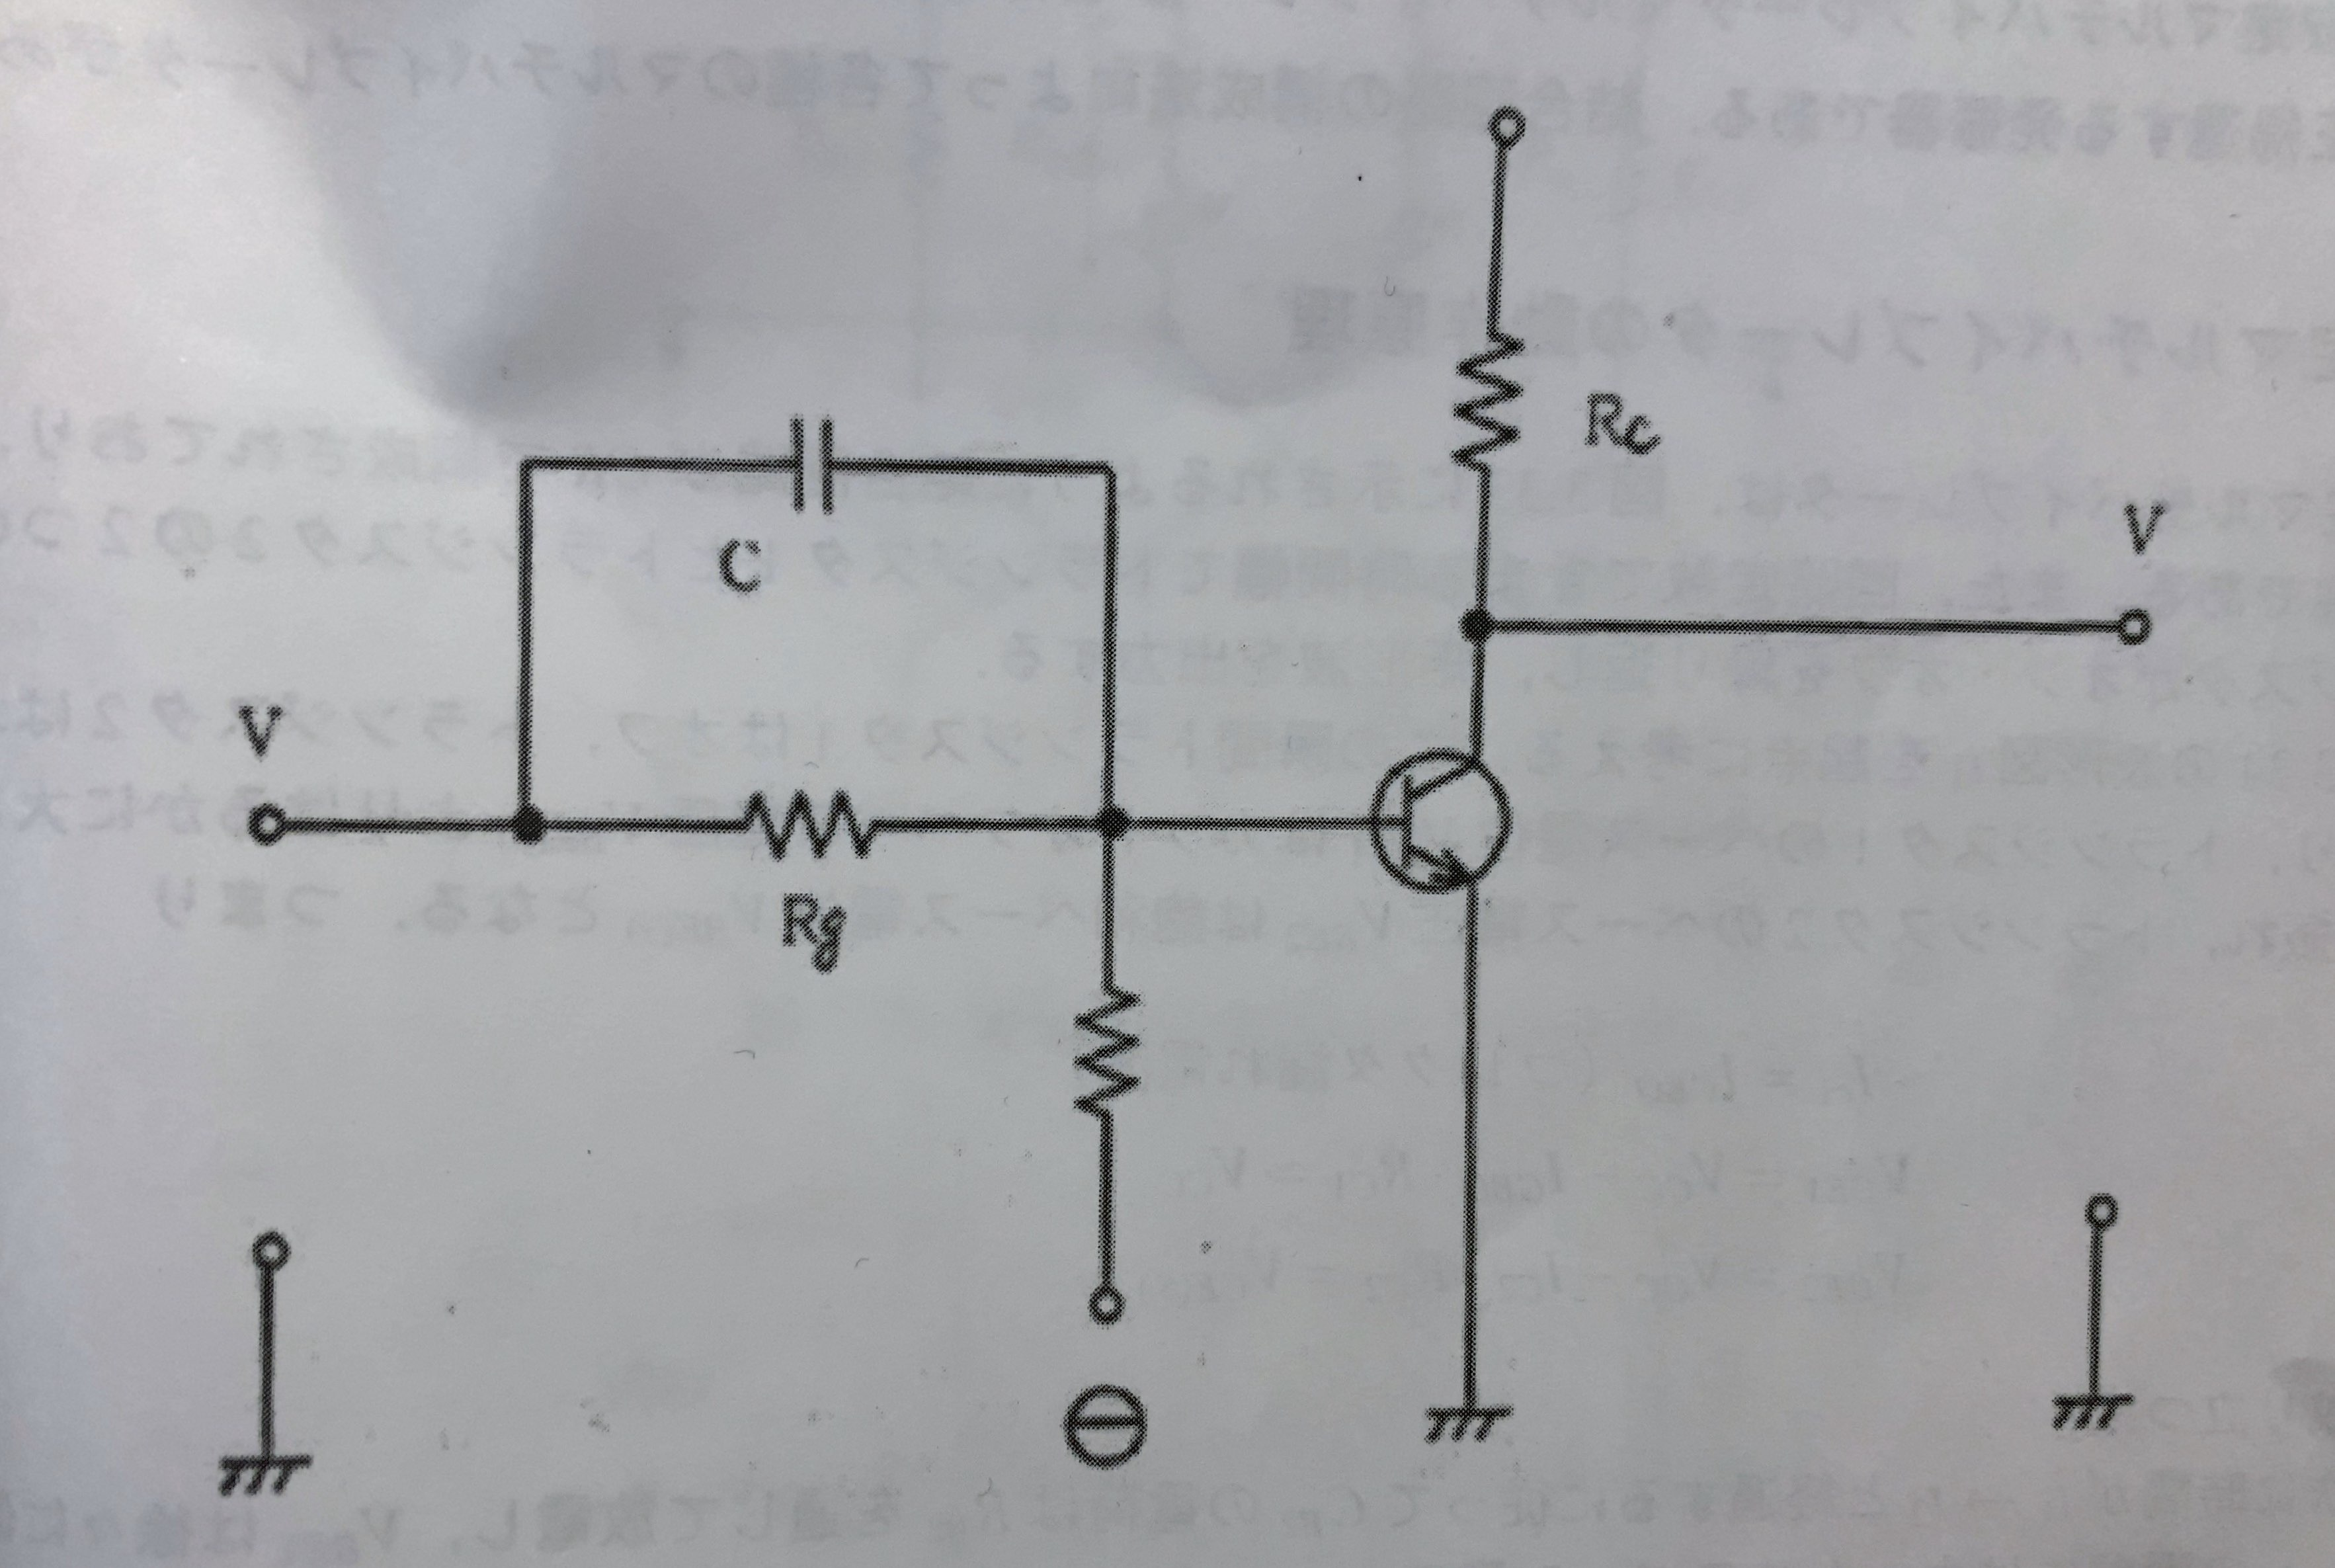
\includegraphics[bb=0 0 3531 2371,height=10cm]{parusu_3.jpg}
    \end{center}
    \caption{スイッチング回路}
    \label{fig3}
    \begin{center}
        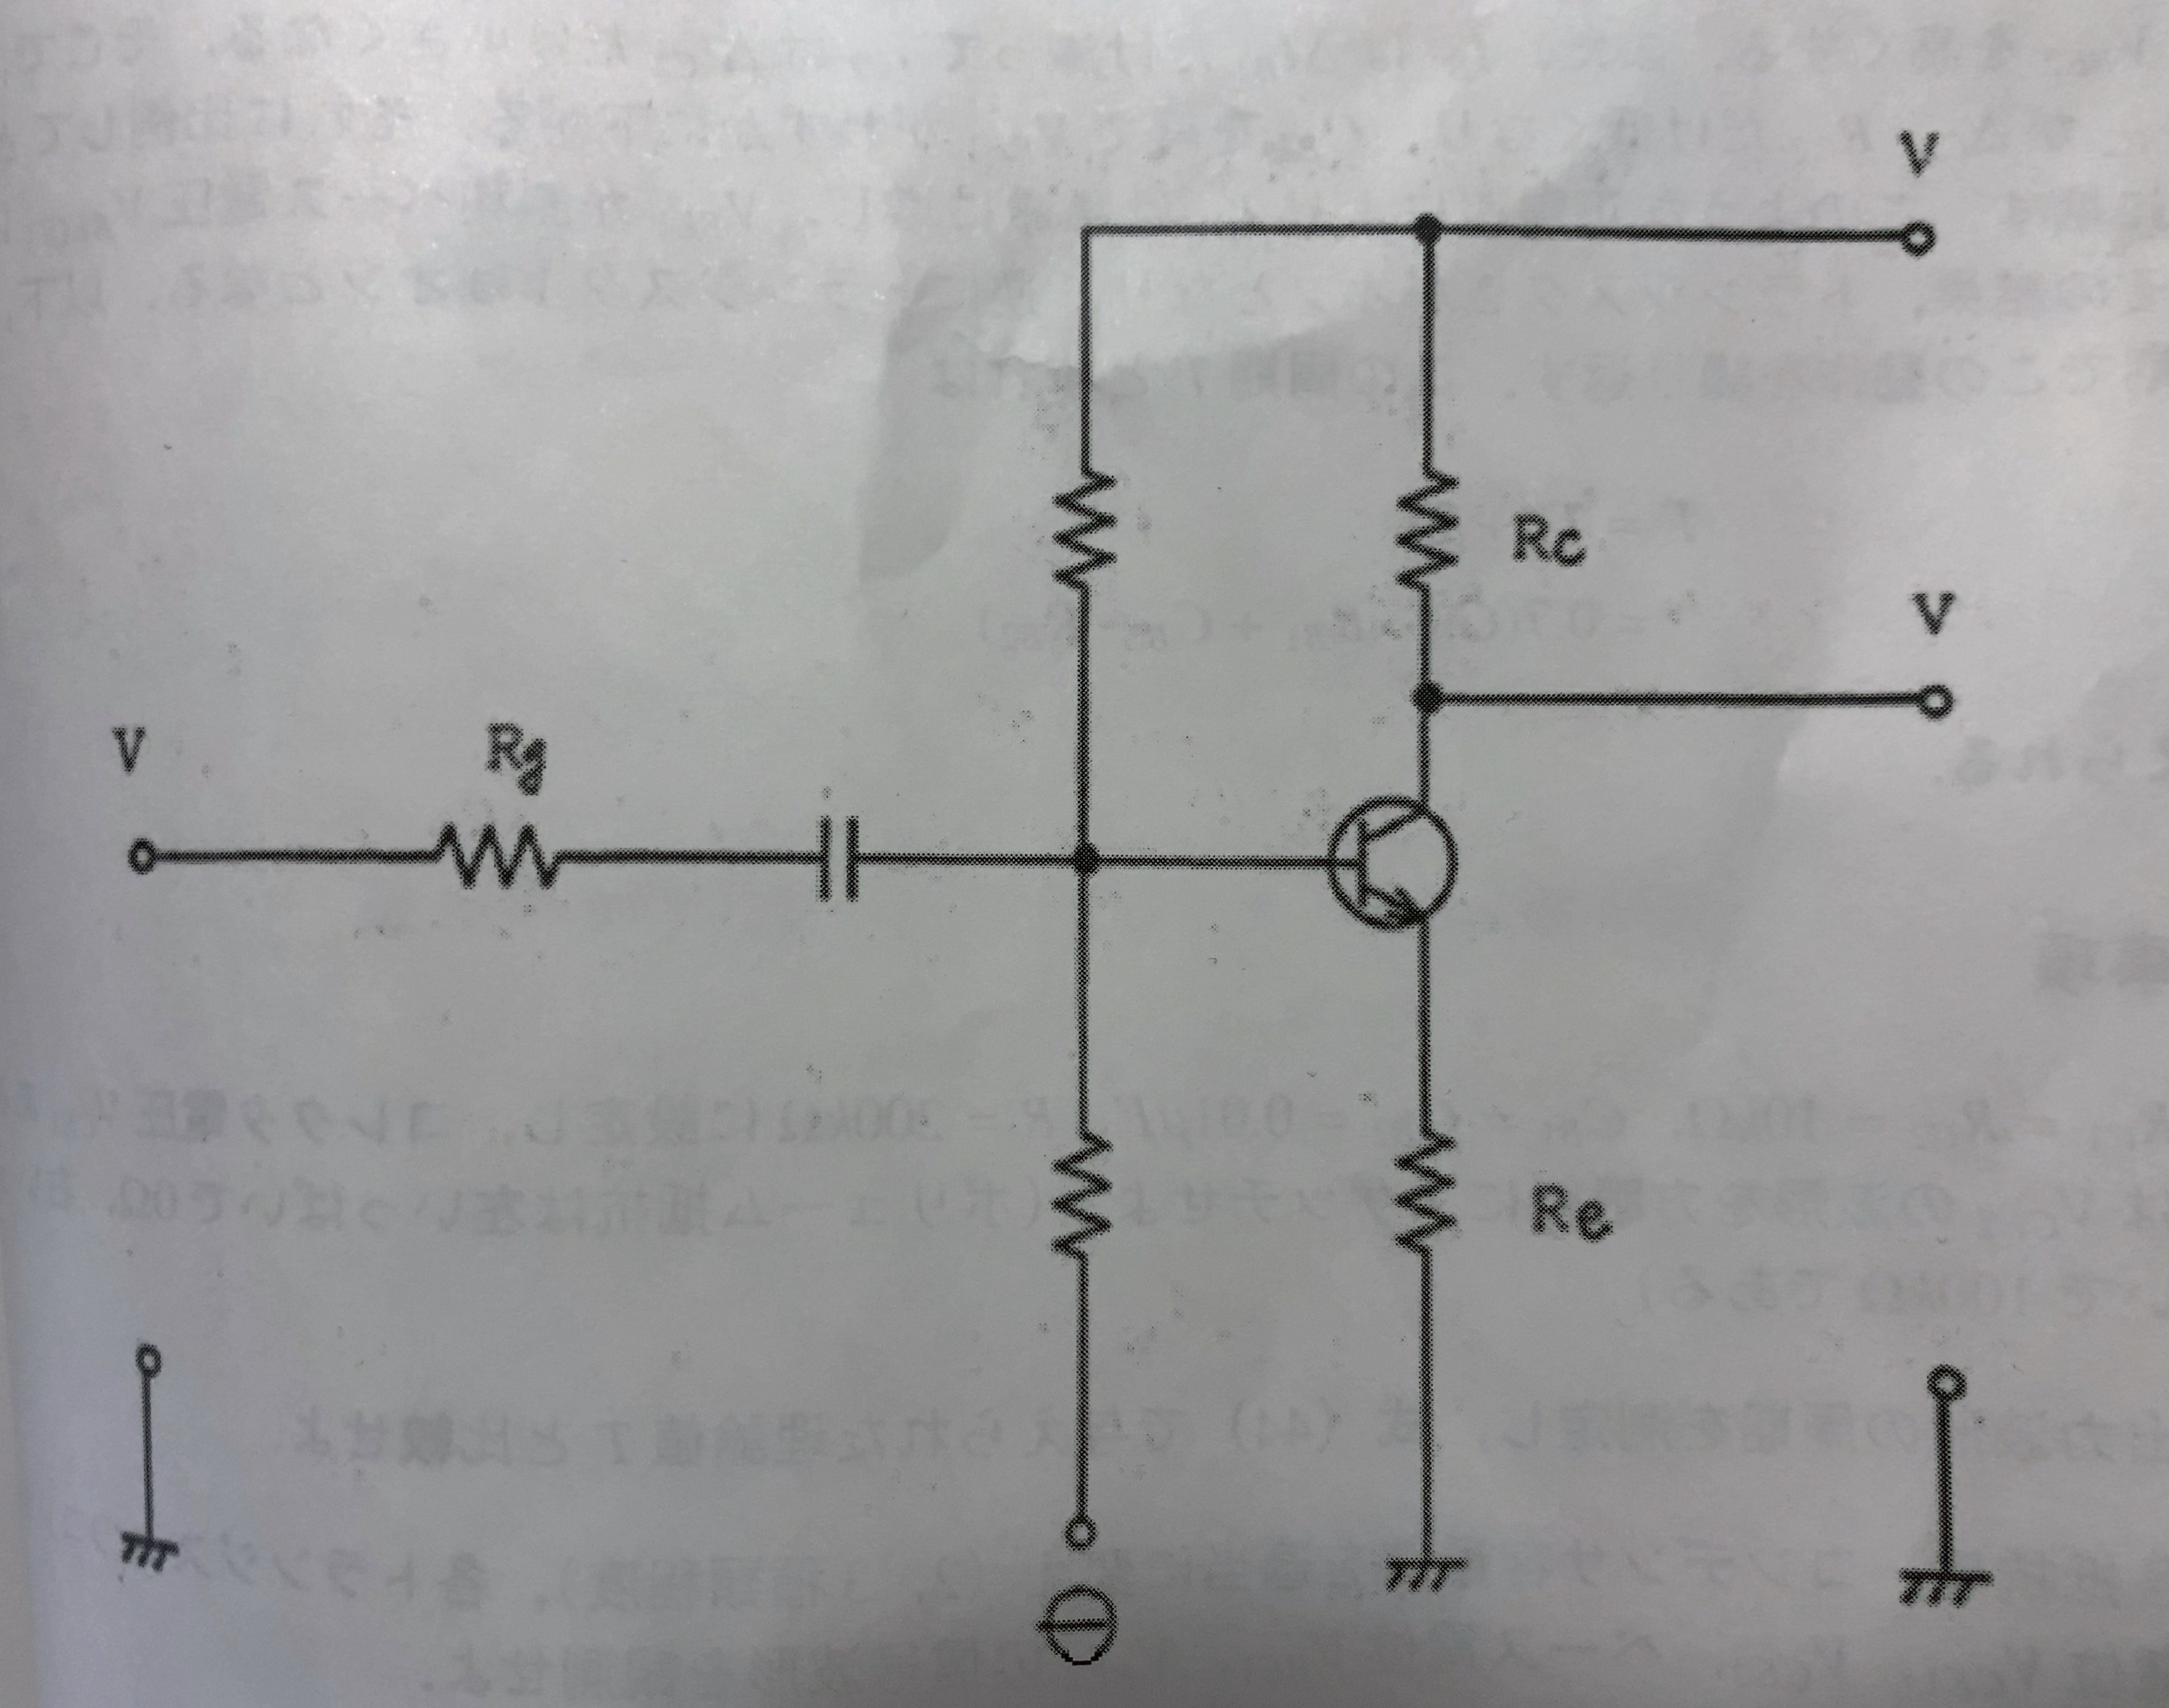
\includegraphics[bb=0 0 3517 2770,height=11cm]{parusu_4.jpg}
    \end{center}
    \caption{パルス増幅回路}
    \label{fig4}
\end{figure}
\clearpage

\subsection{無安定マルチバイブレータ}
無安定マルチバイブレータとは2段の抵抗結合増幅器の出力段から入力段に正帰還する発信器である。
結合回路の構成法によって各種のマルチバイブレータがある。

\subsubsection*{無安定マルチバイブレータの動作原理}
無安定マルチバイブレータは、図\ref{fig5}に示されるように
結合回路が$CR$で構成されており、左右対称である。
また、回数定数できまる時間幅でトランジスタ1とトランジスタ2の
2つのトランジスタがオン・オフを繰り返し、短波形を出力する。

図\ref{fig6}の波形図$t_1$を起点に考える。この瞬間トランジスタ1はオフ、
トランジスタ2はオンとなり、
トランジスタ1のベース電位$V_{BE1}$はカットオフベース電圧$V_{BE(o)}$
よりはるかに大きく正に振れ、
トランジスタ2のベース電位$V_{BE2}$は飽和ベース電位$V_{BE(s)}$となる。
つまり
\begin{eqnarray}
    I_{c1} &=& I_{CBO} (コレクタ漏れ電流)\nonumber\\
    V_{CE1} &=& V_{CC} - I_{CBO} \cdot R_{C1} \simeq V_{CC}\nonumber\\
    V_{CE2} &=& V_{CC} - I_{C2} \cdot R_{C2} = V_{CE(S)}
\end{eqnarray}
が成り立つ。

次に時間が$t_1 \rightarrow t_2$と経過するに従って$C_{B2}$の電荷は
$R_{B2}$を通じて放電し、$V_{BE1}$は徐々に低下し、
$t_2$の瞬間にはカットオフベース電圧$V_{BE(O)}$よりわずかに小さくなる。
このとき、トランジスタ1のベースに微小電流$\Delta I_{B1}$が流れ、
このためコレクタ電流$\Delta I_{C1}$がトランジスタ1に流れる。
従ってトランジスタ1のコレクタ電圧$V_{CE1}$は$\Delta_{C1}\cdot R_{C1}$だけ高くなり、
この電位は$C_B$を通じて$V_{BE2}$を高くする。
また、$I_{B2}$は$\Delta I_{B2}$だけ減って$I_{C2}$は$\Delta I_{C2}$だけ小さくなる。
そこで、今度は$V_{CE2}$が$\Delta_{C2}\cdot R_{C2}$だけ低くなり、
$C_{B2}$を経て$V_{BE1}$がわずかに下がる。
それに比例して$\Delta I_{B1}$がさらに増す。
このような正帰還により$I_{B1}$は急激に増し、$V_{BE1}$が飽和ベース電圧$V_{BE(S)}$に達する。
その結果、トランジスタ2がオフとなり、逆にトランジスタ1はオンとなる。
以下、一定の周期でこの動作を繰り返す。この周期$T$とすれば
\begin{eqnarray}
    T &=& T_1 + T_2\nonumber\\
    &=& 0.7(C_{B1} \cdot R_{B1} + C_{B2} \cdot R_{B2}) \label{eq3}
\end{eqnarray}
で与えられる。

\subsubsection*{実験事項}
\begin{enumerate}
    \item $R_{C1} = R_{C2} = 10k\Omega$、$C_{B1} = C_{B2}= 0.01 \mu F$、
          $R = 200k\Omega$に設定し、
          コレクタ電圧$V_{CE1}$あるいは$V_{CE2}$の波形を観測する。
          (ボリューム抵抗は左いっぱいで$0\Omega$、右いっぱいで$100k\Omega$である)
    \item 出力波形の周期を測定し、式(\ref{eq3})で与えられた理論値$T$と比較する。
    \item 各抵抗値、コンデンサ容量値を適当に変え (2、3種類程度)、
          各トランジスタのコレクタ電位$V_{CE1}$、$V_{CE2}$、
          ベース電位$V_{BE1}$、$V_{BE2}$の信号波形を観測する。
\end{enumerate}

\clearpage
\begin{figure}[h]
    \begin{center}
        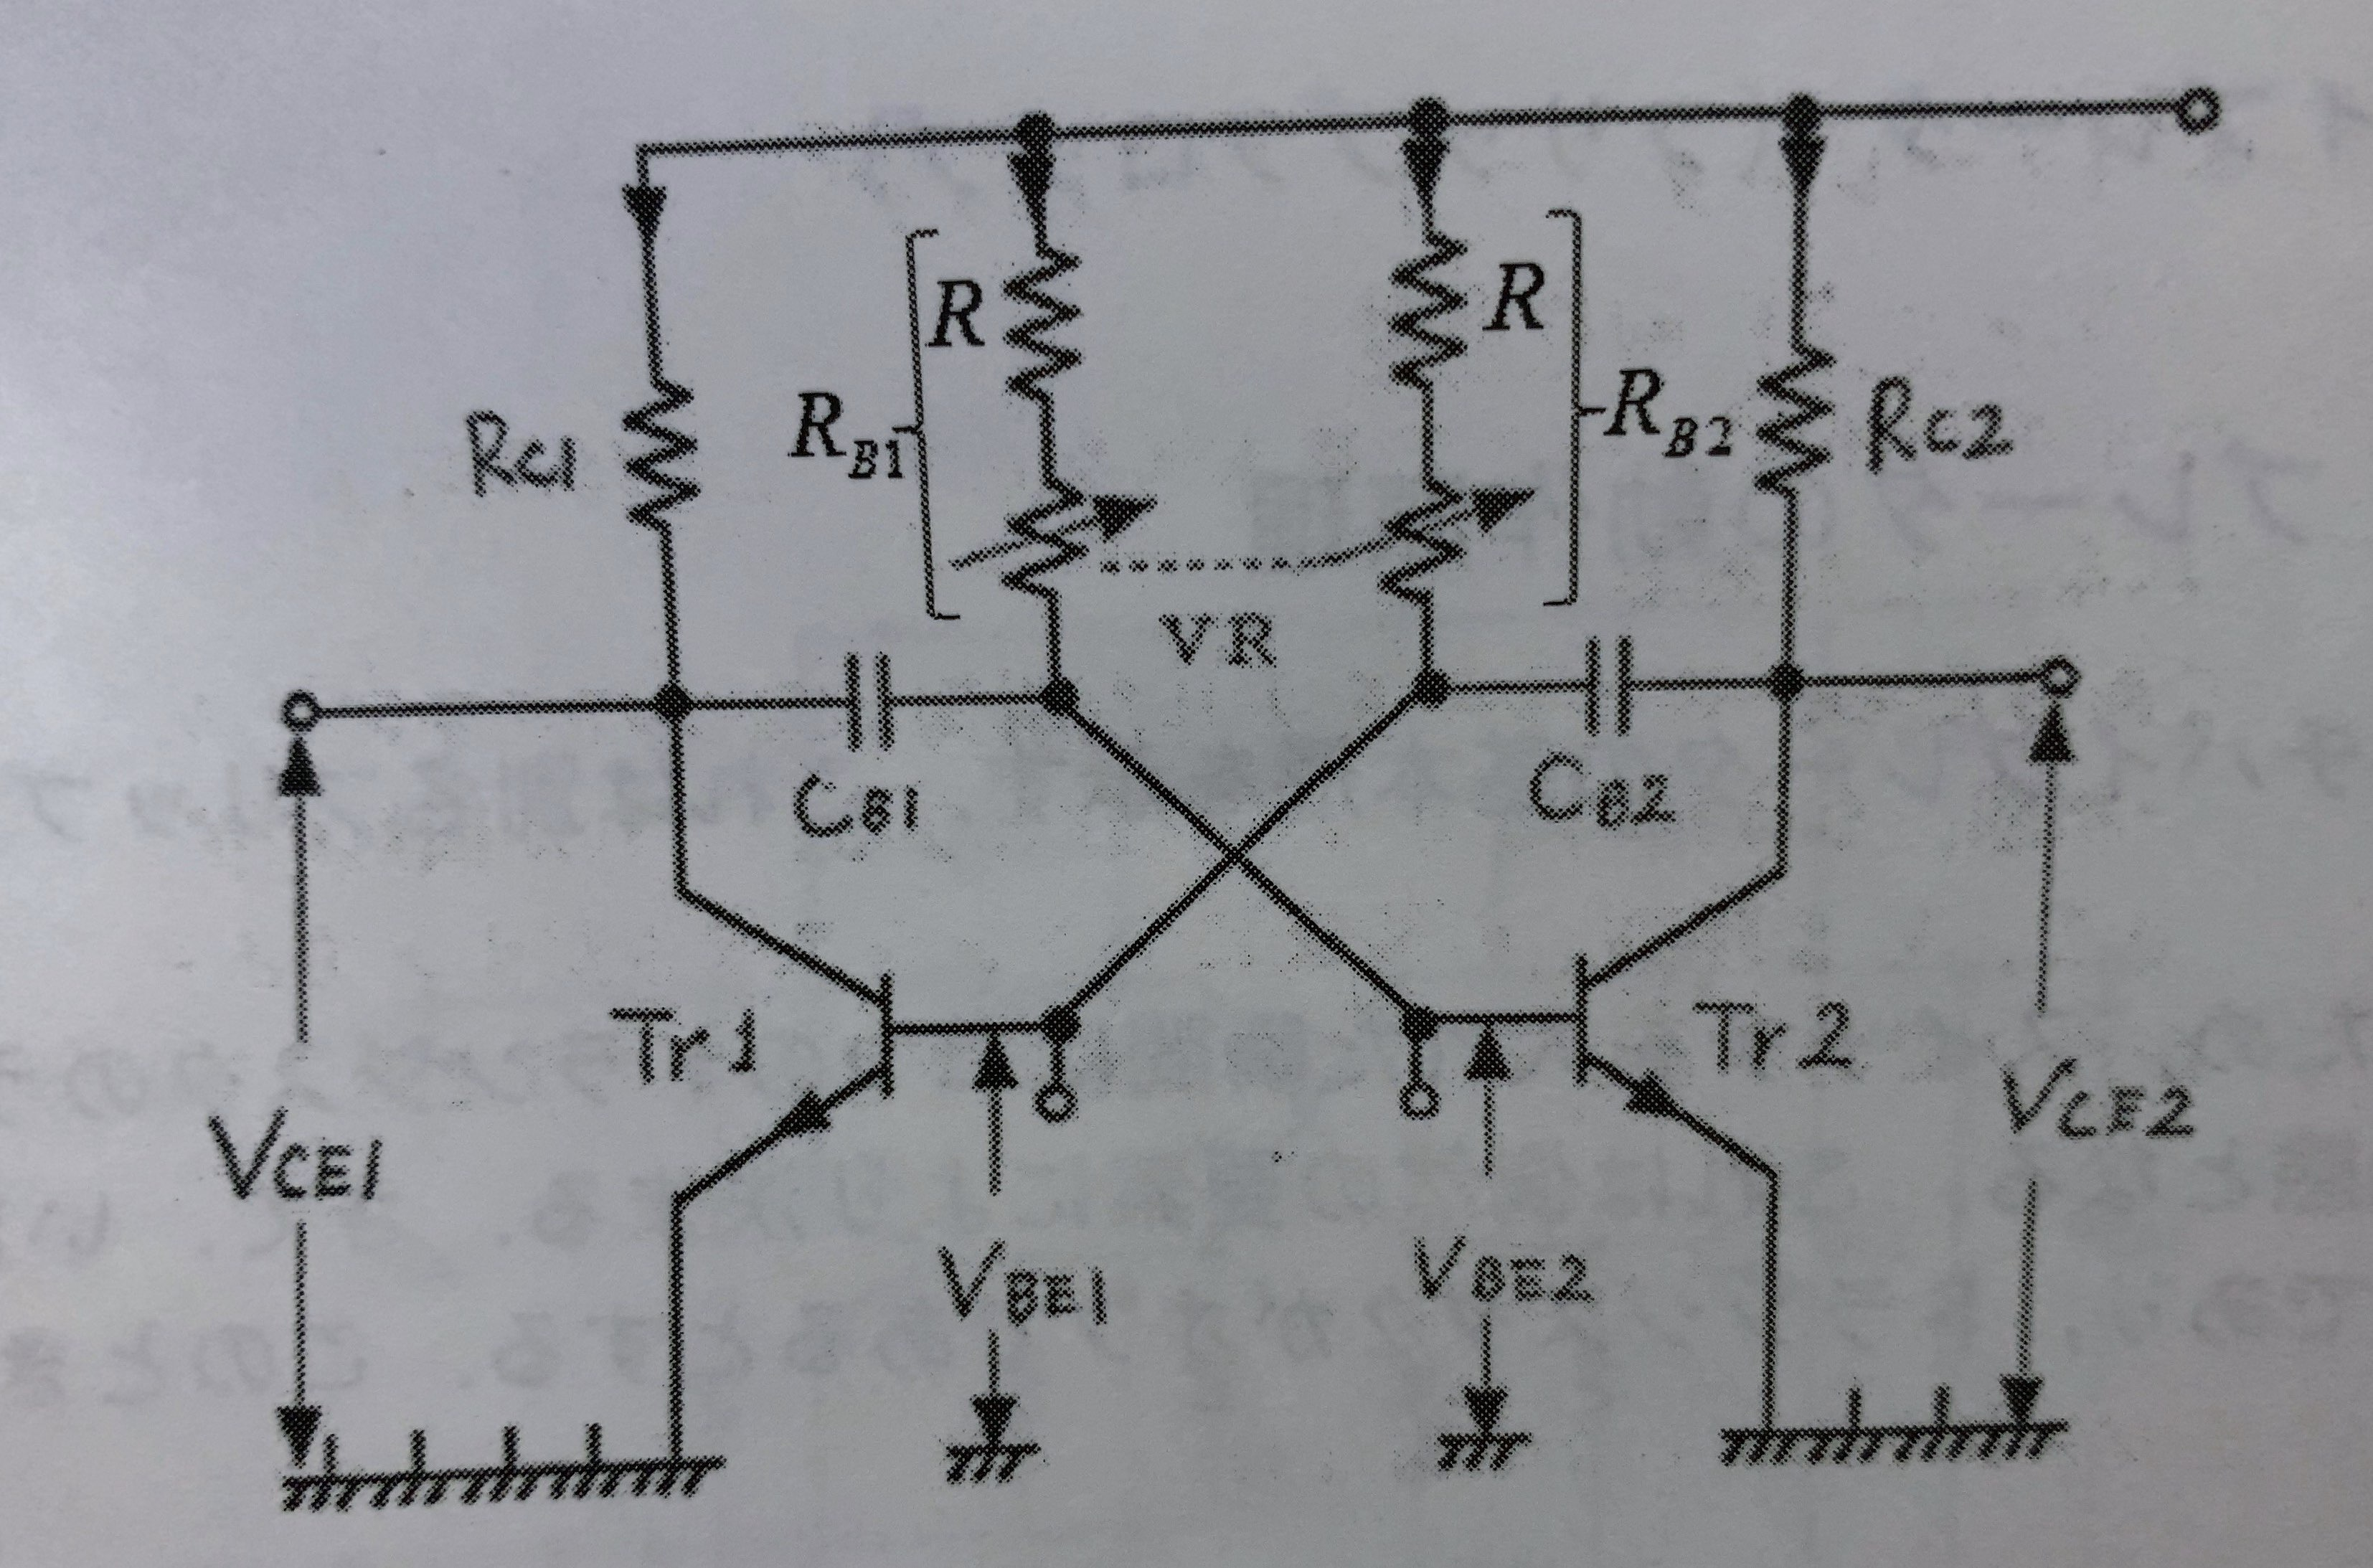
\includegraphics[bb=0 0 3308 2186,height=10cm]{parusu_5.jpg}
    \end{center}
    \caption{無安定マルチバイブレータ}
    \label{fig5}
    \begin{center}
        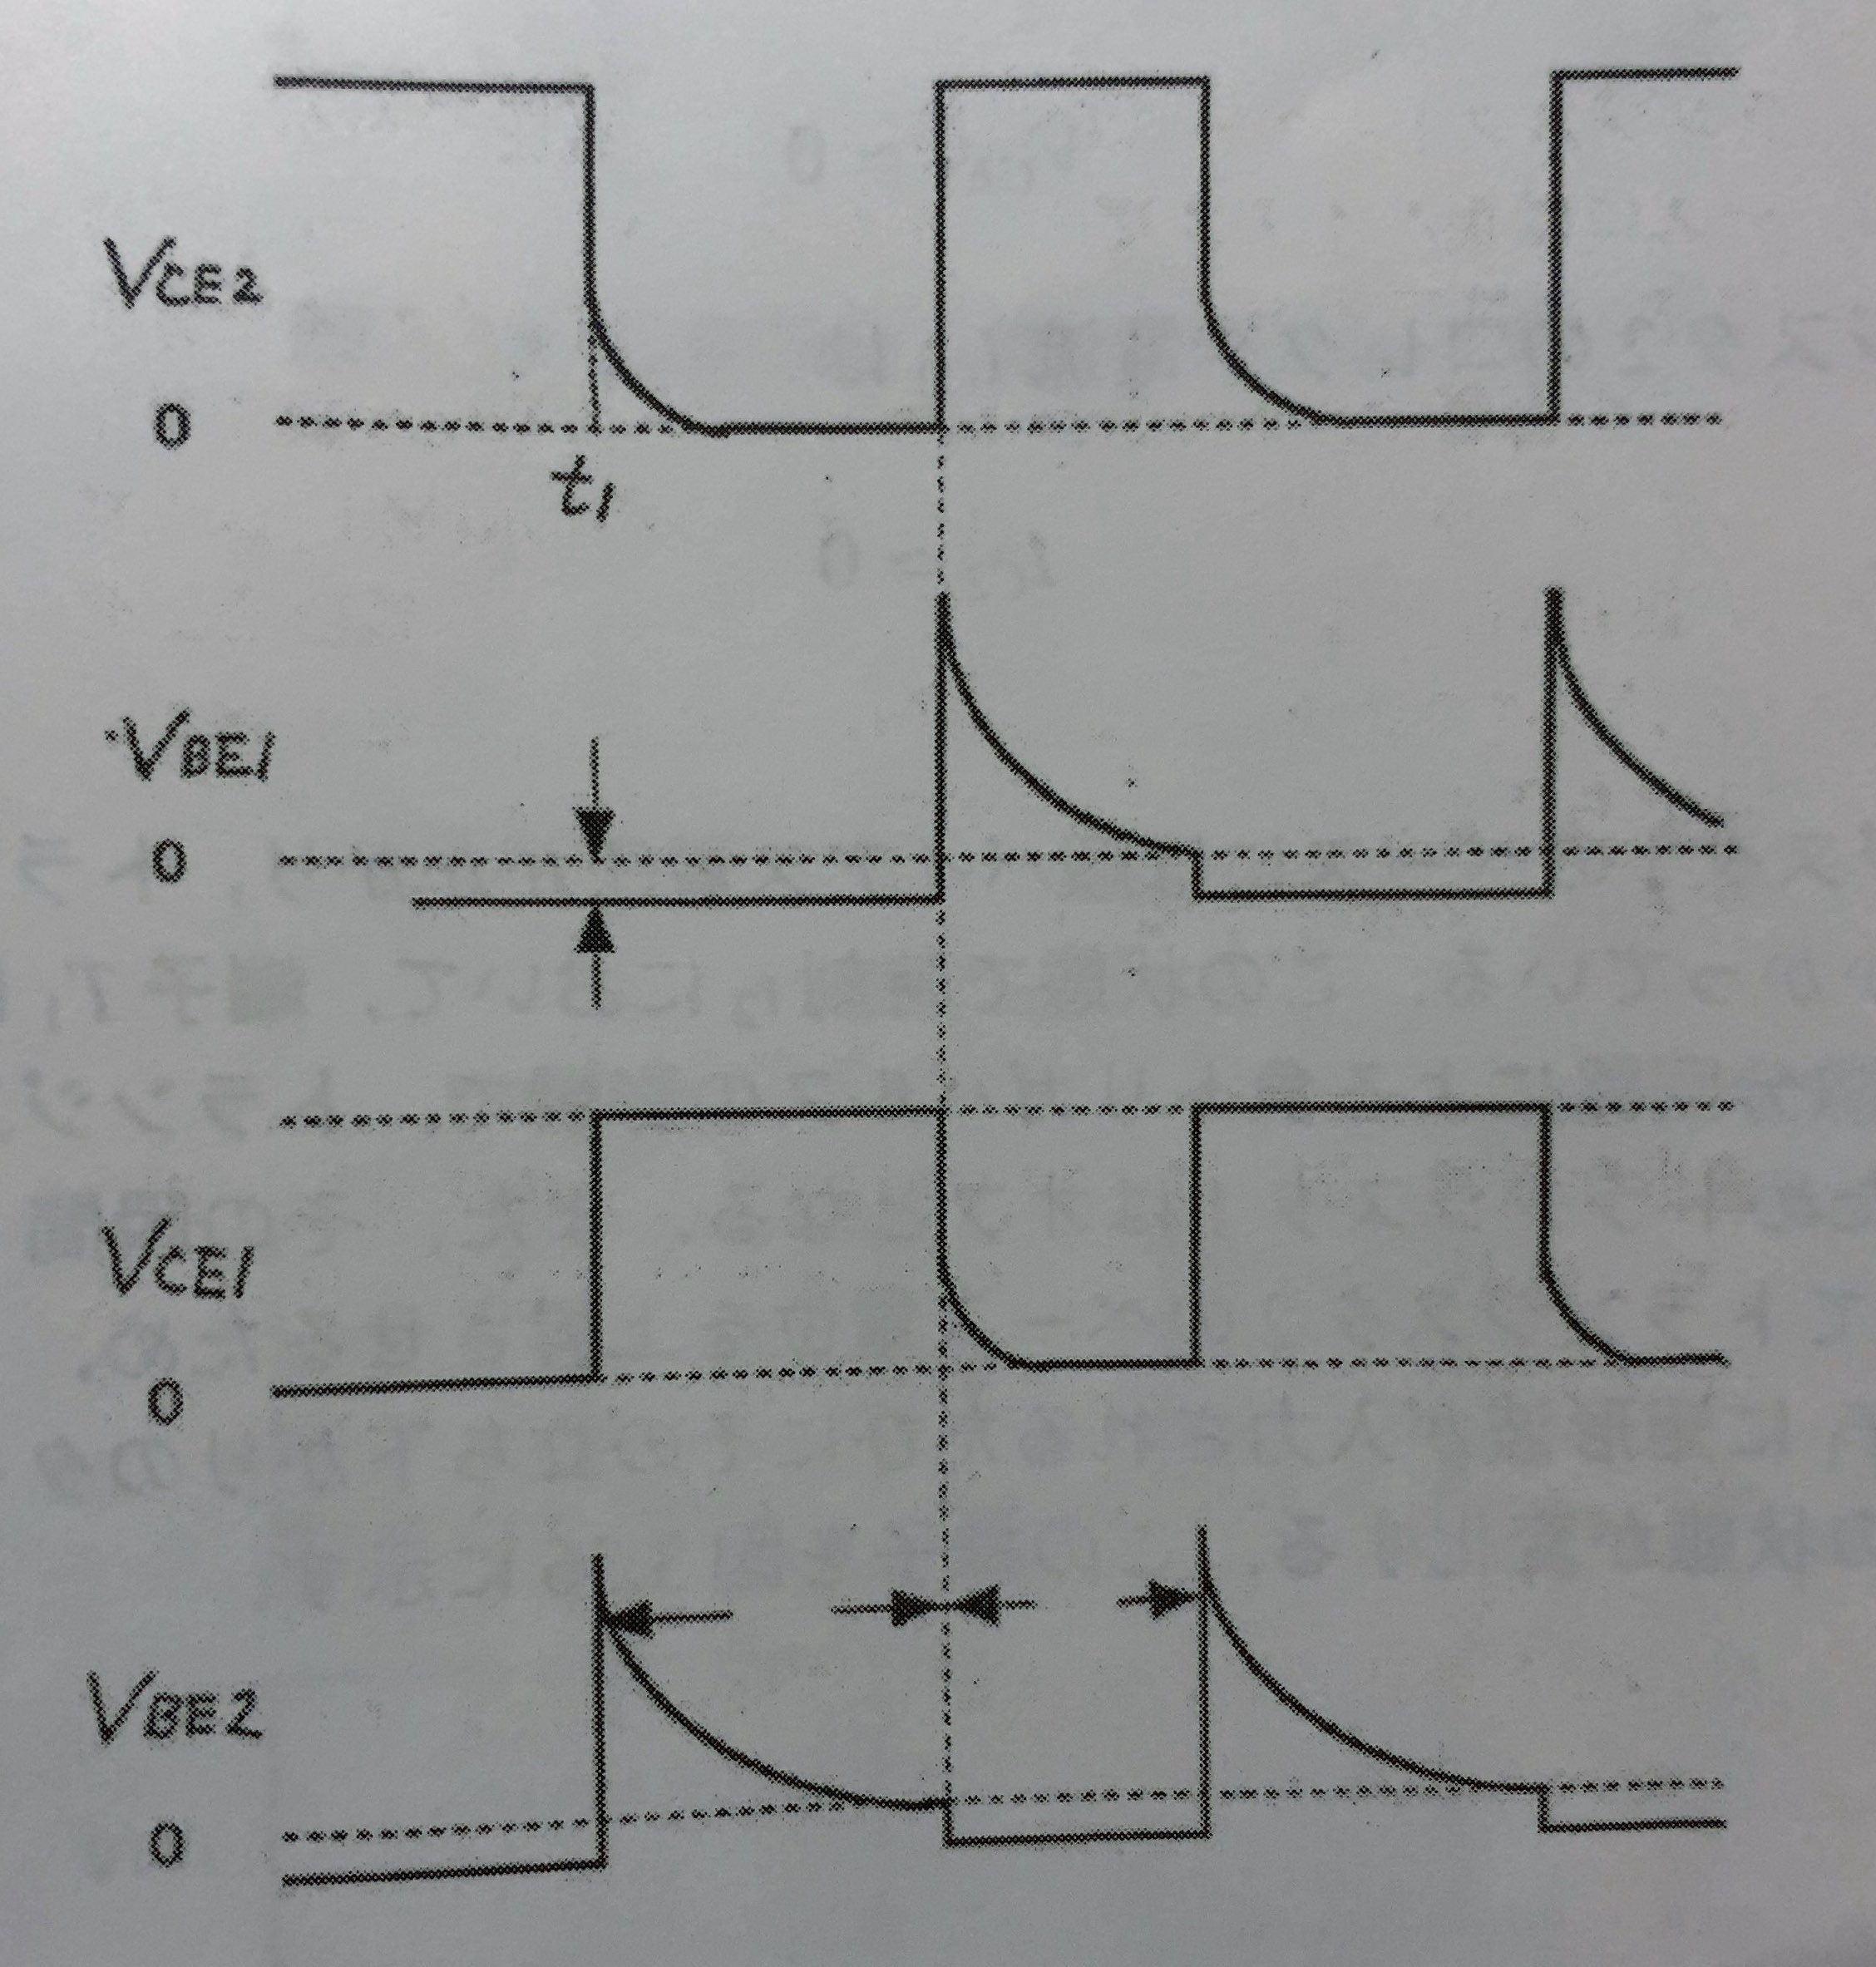
\includegraphics[bb=0 0 2256 2366,height=10cm]{parusu_6.jpg}
    \end{center}
    \caption{無安定マルチバイブレータ 各部の波形図}
    \label{fig6}
\end{figure}
\clearpage

\subsection{双安定マルチバイブレータ(フリップフロップ)}
\subsubsection*{双安定マルチバイブレータの動作原理}
図\ref{fig7}に双安定マルチバイブレータの基本形を示す。
これは別名フリップフロップと呼ばれることもある。

回路は対称であるため、
スイッチを入れた瞬間は二つのトランジスタのうち片方がオン状態、もう片方がオフの状態となる。
これは偶然の要素により決まる。
さて、いま時刻$t_1$の瞬間にトランジスタ1がオンであり、
トランジスタ2がオフであるとする。
このとき、トランジスタ2のコレクタ電圧は
\begin{eqnarray}
    V_{CE2} \simeq V_{CC}\nonumber
\end{eqnarray}
となり、トランジスタ1のコレクタ電圧は
\begin{eqnarray}
    V_{CE1} \simeq 0\nonumber
\end{eqnarray}
となる。またトランジスタ2のコレクタ電流$I_{C2}$は
\begin{eqnarray}
    I_{C2} \simeq 0\nonumber
\end{eqnarray}
である。

このとき、トランジスタ1のベースには順バイアス電圧がかかり、
トランジスタ2のベースには逆バイアス電圧がかかっている。
この状態で時刻$t_2$において、端子$T_1$に短形波を入力すると
$C_1$、$R_1$で構成される微分回路による負トリガパルスの影響で、
トランジスタ1のベース電位が負の電位に振られるためトランジスタ1はオフとなる。
また、その瞬間$V_{CE1}$の電位が上昇し、
それが抵抗$R_3$を通じてトランジスタ2のベース電位を上昇させるため、トランジスタ2はオンとなる。
以後、端子$T_1$に短形波が入力されるたびにその立ち下がりのタイミングで、
各トランジスタのオン・オフの状態が変化する。この様子を図\ref{fig8}に示す。

\subsubsection*{実験事項}
\begin{enumerate}
    \item $T_1$に適当な振幅(例えば、$10(V)$程度)と発振周波数(例えば、$1kHz$程度)
          を持つ無安定マルチバイブレータの出力を入力させ、
          各トランジスタのコレクタ電位$V_{CE1}$、$V_{CE2}$と
          ベース電位$V_{BE1}$、$V_{BE2}$波形を観測する。
          ただし、入力端子$T_1$へ入力電圧は$10\sim12(V)$程度とし、
          $R_{C1}=R_{C2}=2k\Omega$、$C_3=C_4=100pF$と
    \item $R_{C1}$、$R_{C2}$、$C_3$、$C_4$の値を適当に変えて上記と同様の測定を行え。
          ただし、$R_{C1}=R_{C2}$、$C_3=C_4$とすること。
\end{enumerate}

\clearpage
\begin{figure}[h]
    \begin{center}
        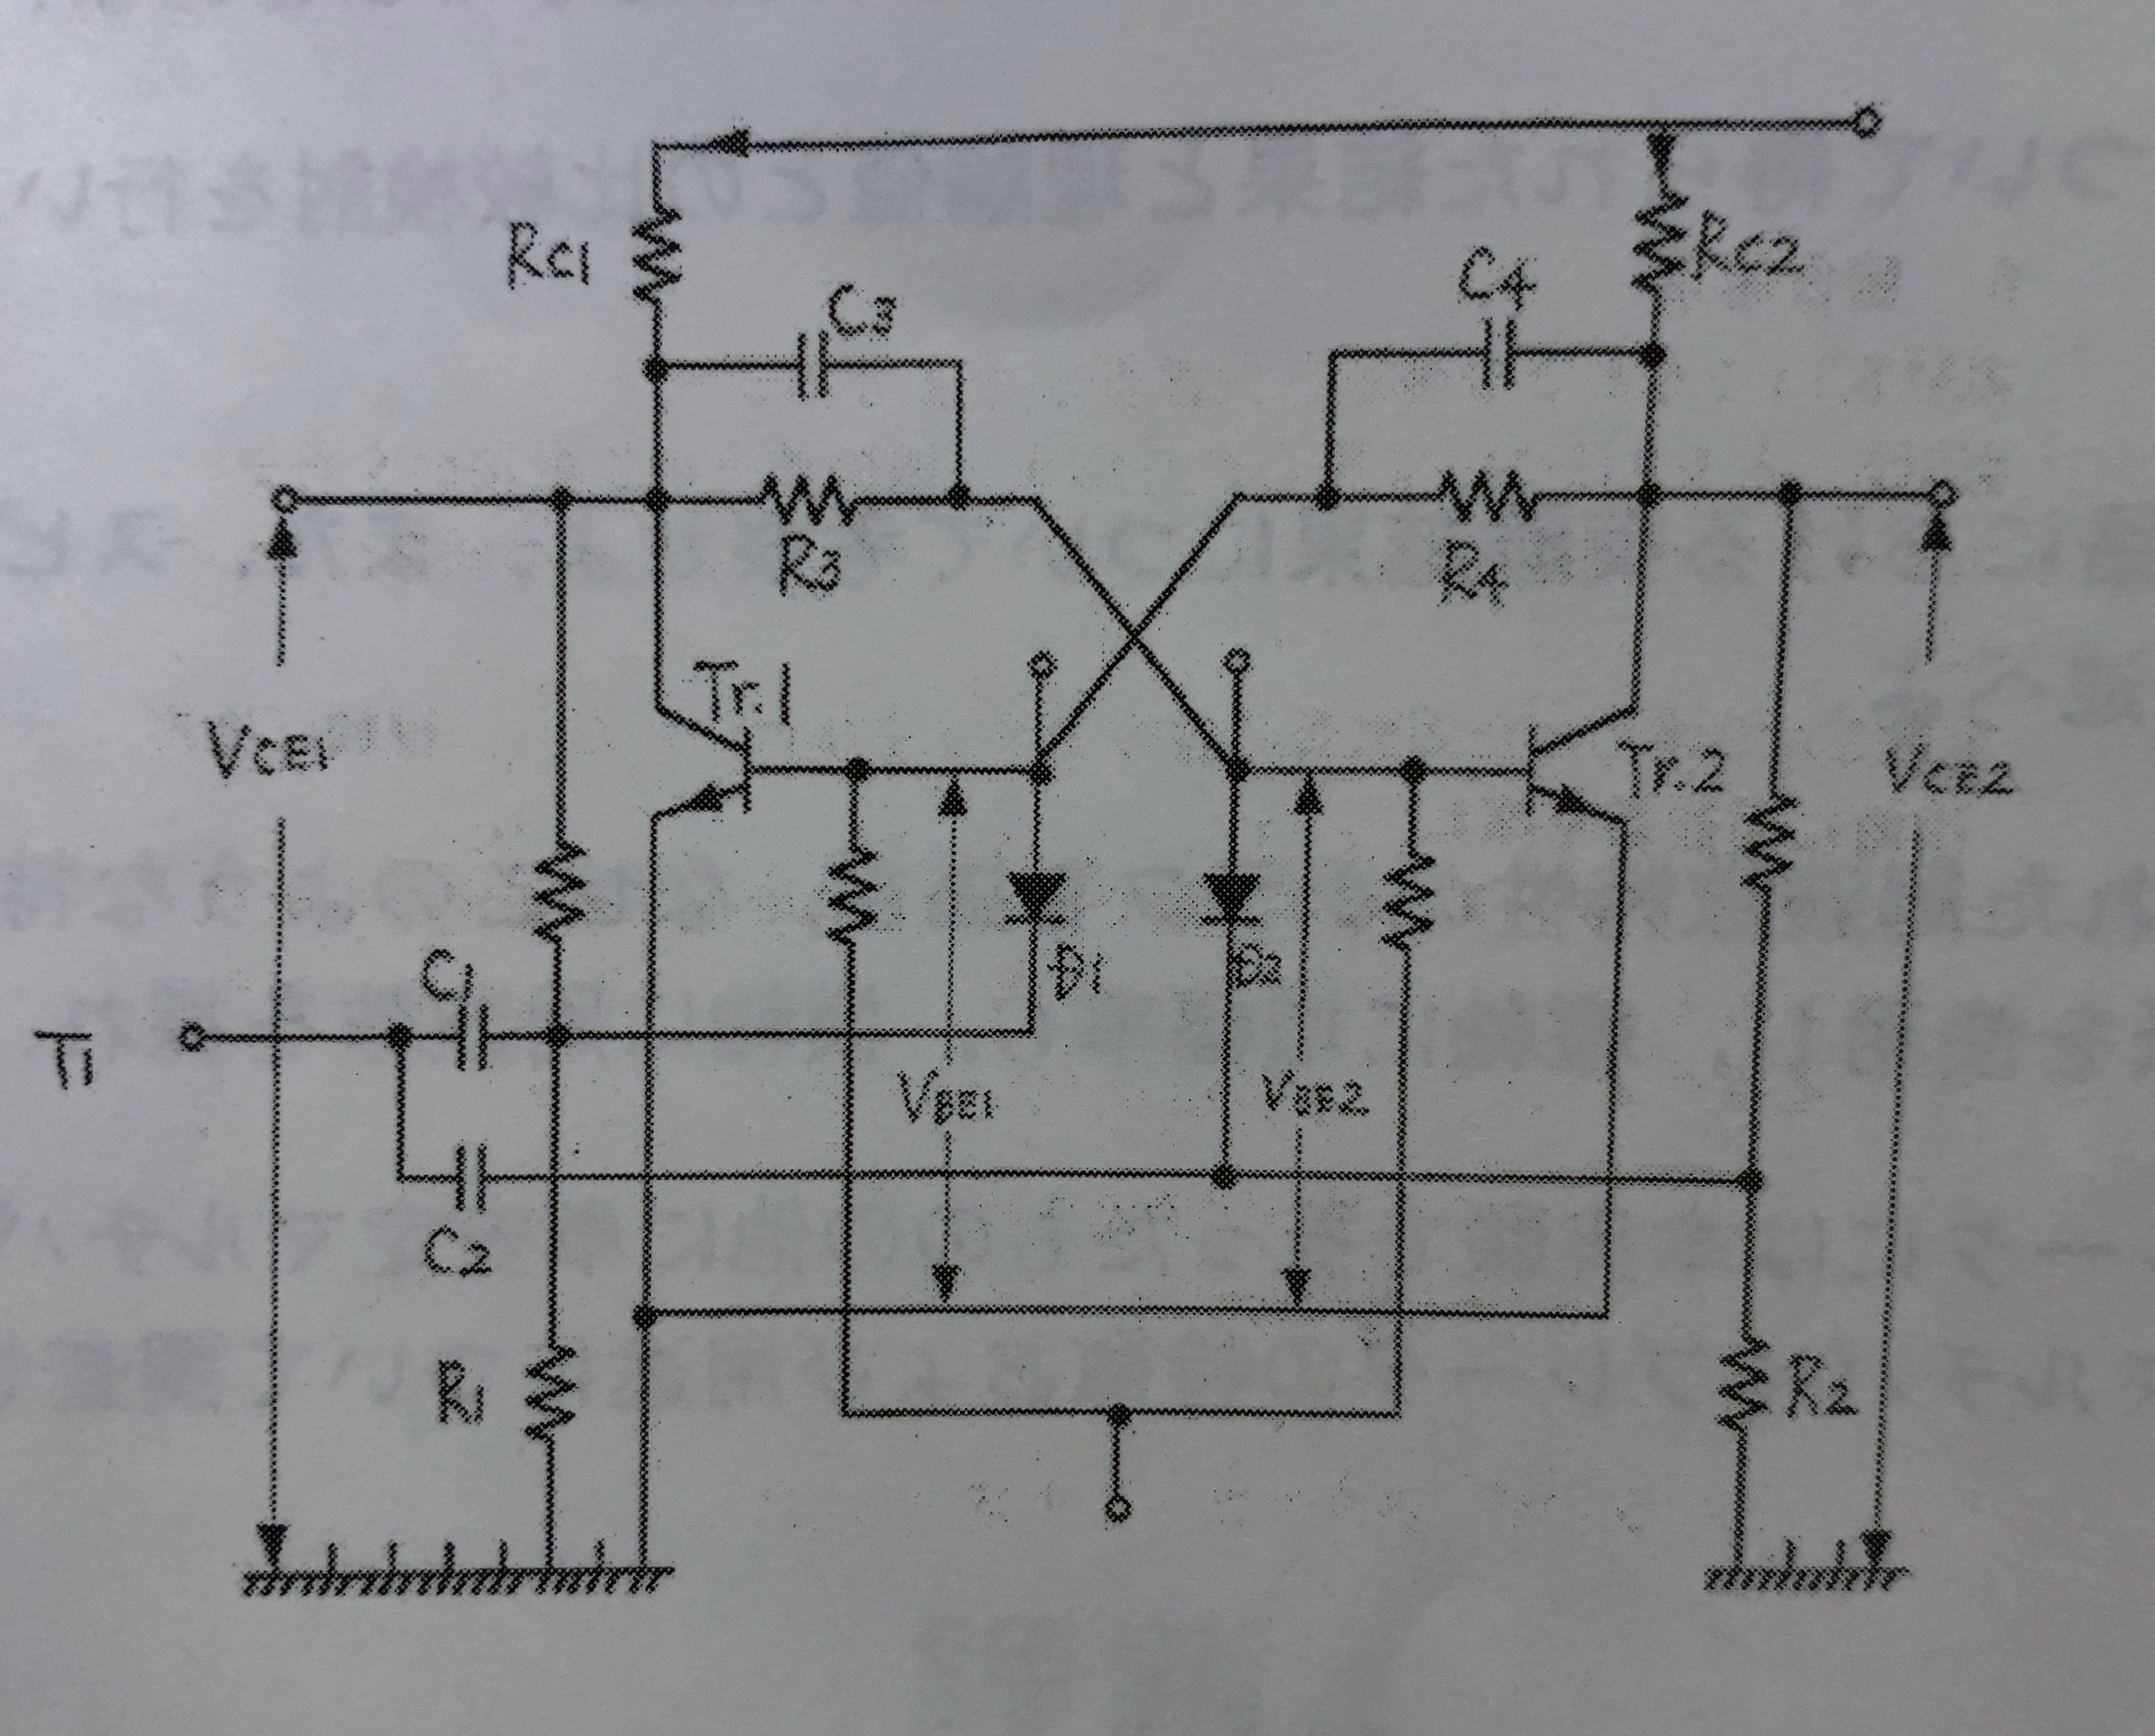
\includegraphics[bb=0 0 2945 2373,height=11cm]{parusu_7.jpg}
    \end{center}
    \caption{双安定マルチバイブレータ}
    \label{fig7}
    \begin{center}
        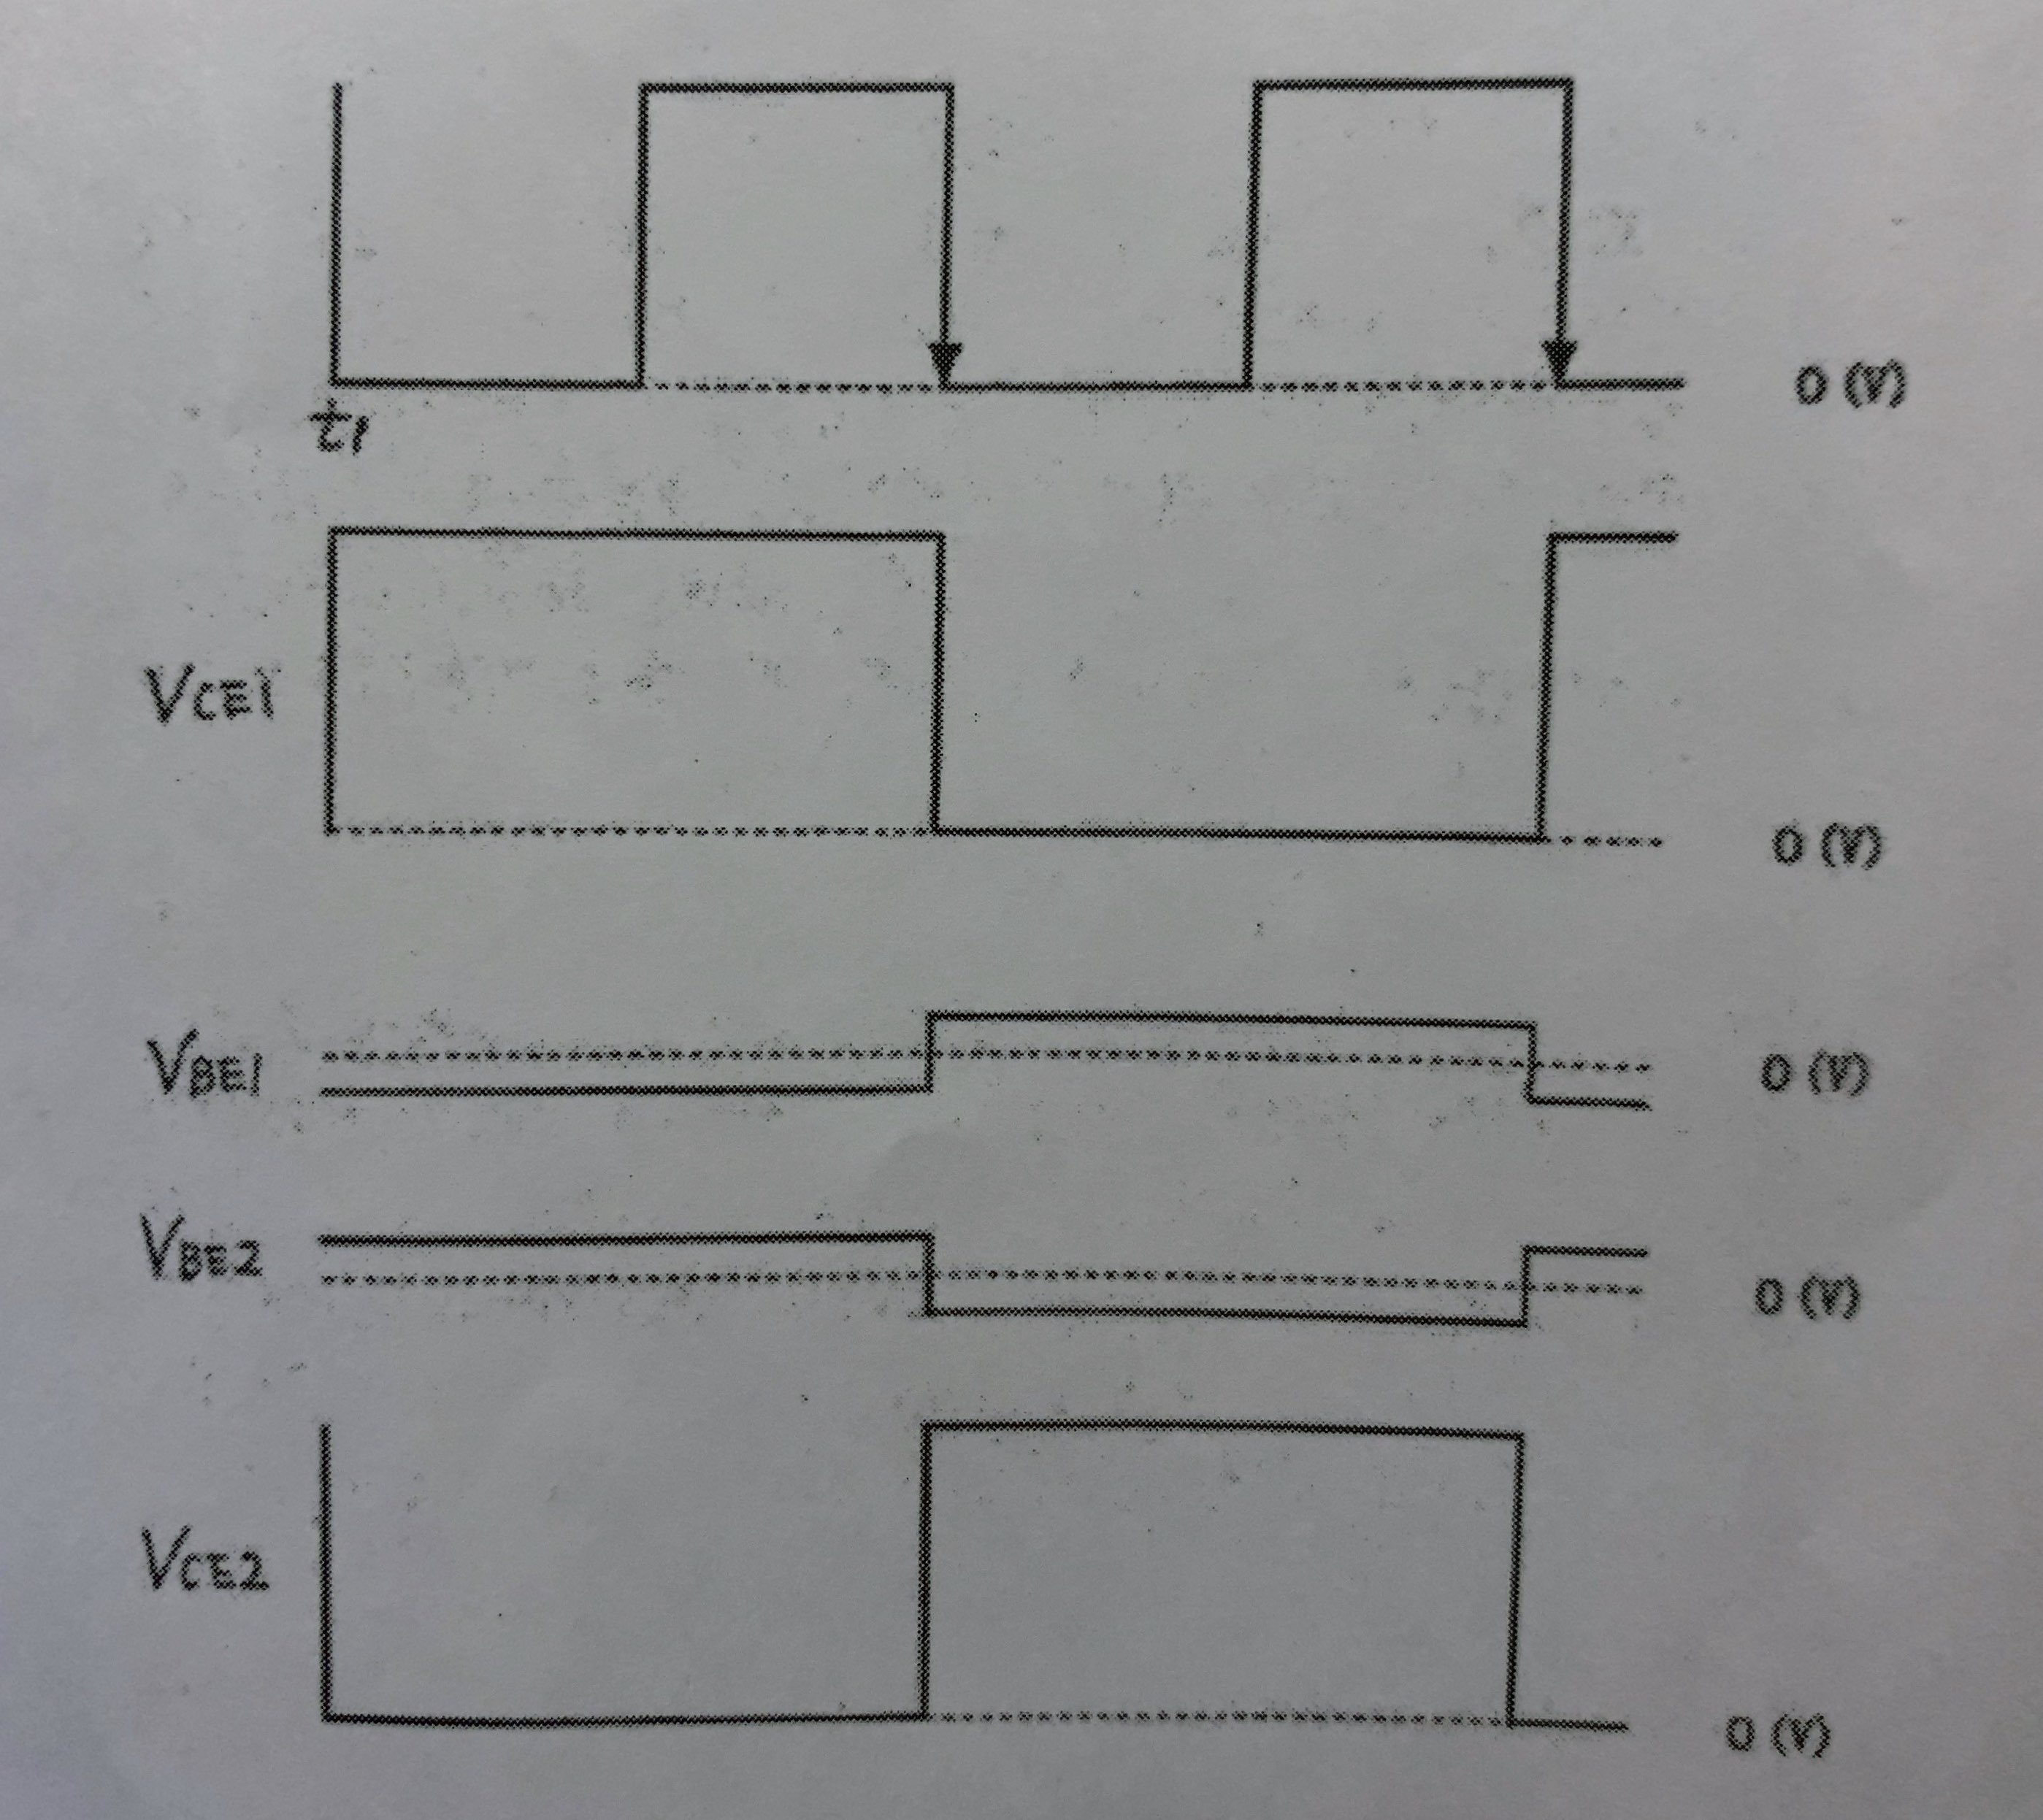
\includegraphics[bb=0 0 2798 2493,height=11cm]{parusu_8.jpg}
    \end{center}
    \caption{双安定マルチバイブレータ 各部の波形図}
    \label{fig8}
\end{figure}
\clearpage

\section{検討・考察}

\subsection{レポート課題1}
\begin{shadebox}
    テキスト中の図3.29は微分回路を示している。
    この回路では入力信号$e(t)$を印加したときに、
    $R$の両側で観測される電圧が$v(t)$であるとき、
    $v(t)$の近似値は$e(t)$を微分した量で与えられる。
    その根拠について考察せよ。
\end{shadebox}
コンデンサにかかる電圧を$V_C(t)$として電流を$i$として、
与えられた文字(抵抗の電圧$v(t)$と入力信号$e(t)$)を用いる。

まず、コンデンサにかかる電圧$V_C(t)$と抵抗の電圧$v(t)$は、
次式(4)、(5)のように表せる。
\begin{eqnarray}
    V_C(t)&=&\frac{\int idt}{C}\\
    v(t)&=&Ri
\end{eqnarray}
キルヒホッフの法則より
\begin{eqnarray}
    e(t)&=&v(t)+V_C(t)
\end{eqnarray}
したがって、式(4)、(5)を代入して、
\begin{eqnarray}
    e(t)&=&Ri+\frac{\int idt}{C}
\end{eqnarray}
式(7)の両辺を$t$で微分すると、
\begin{eqnarray}
    0&=&R\frac{di}{dt}+\frac{i}{C}
\end{eqnarray}
そして、定数分離して微分方程式を解きやすい形にすると、
\begin{eqnarray}
    \frac{1}{i}\frac{di}{dt}&=&-\frac{1}{CR}
\end{eqnarray}
電流$i$を求めるために式(9)の両辺を$t$で積分すると、
\begin{eqnarray}
    \int \frac{1}{i} \frac{di}{dt}dt&=&\int-\frac{1}{CR}dt \nonumber\\
    \int \frac{1}{i}di&=&-\frac{1}{CR}\int dt \nonumber\\
    log_e|i|&=&-\frac{1}{CR}+X \nonumber\\
    i&=&e^{-\frac{t}{CR}+X} \nonumber\\
    i&=&e^Xe^{-\frac{t}{CR}}(Xは積分定数)
\end{eqnarray}
\clearpage

初期条件「$t=0$のとき、$V_C(t)=0$」なので、
式(6)、(7)より、
\begin{eqnarray}
    「t=0のとき、V_C(t)=0」&\Leftrightarrow& 「t=0のとき、e(t)=v(t)」\nonumber\\
    &\Leftrightarrow&「t=0のとき、e(t)=Ri」\nonumber\\
    &\Leftrightarrow&「t=0のとき、i=\frac{e(t)}{R}」
\end{eqnarray}
である。これを、式(10)に代入して、
\begin{eqnarray}
    \frac{e(t)}{R}&=&e^Xe^{-\frac{0}{CR}}\nonumber\\
    \frac{e(t)}{R}&=&e^X
\end{eqnarray}
となるので、回路を流れる電流$i$は
\begin{eqnarray}
    i&=& \frac{e(t)}{R}e^{-\frac{t}{CR}}
\end{eqnarray}
となる。したがって、抵抗にかかる電圧$v(t)$は
\begin{eqnarray}
    v(t)=Ri=e(t)e^{-\frac{t}{CR}}
\end{eqnarray}
となり、 $v(t)$の近似値は$e(t)$を微分した量で与えられることが分かる。

\subsection{レポート課題2}
\begin{shadebox}
    テキスト中の図3.30は積分回路である。
    1.と同様に入力信号$e(t)$を印加したとき、
    $C$の両側で観測される電圧$v(t)$の近似値は$e(t)$を積分することにより与えられる。
    その根拠について考察せよ。
\end{shadebox}
この課題で扱う回路はレポート課題1の回路において$R$と$C$の位置を替えたものであるから、
今回は抵抗の電圧を$V_R(t)$、コンデンサにかかる電圧を$V_C(t)$とすると、
レポート課題1の式(4)、(5)は次のように変形できる。
\begin{eqnarray}
    v(t)&=&\frac{\int idt}{C}\\
    V_R(t)&=&Ri
\end{eqnarray}
この後は、レポート課題1の式(6)~(13)のように同様にして、$i$を導くと、
\begin{eqnarray}
    i&=& \frac{e(t)}{R}e^{-\frac{t}{CR}}
\end{eqnarray}
となるので、$v(t)$は
\begin{eqnarray}
    v(t)&=&\frac{\int e(t)e^{-\frac{t}{CR}}dt}{CR}\nonumber
\end{eqnarray}
となり、$v(t)$の近似値は$e(t)$を積分することにより与えられることが分かる。

\clearpage

\subsection{レポート課題3}
\begin{shadebox}
    スイッチング回路における実験結果について考察せよ。
    また、スピードアップコンデンサの効果について述べよ。
\end{shadebox}
\subsubsection*{スピードアップコンデンサ無し}
スピードアップコンデンサ無しでトランジスタを使用すると応答時間が遅れてしまうので、
ONにしたとき、遅延によって高速なスイッチングはできない。
また、OFFにしたときは、トランジスタが飽和することにより、
ベースに蓄えられる電荷も加わるため、更に遅くなる。

\subsubsection*{スピードアップコンデンサ有り(スピードアップコンデンサの効果)}
電源をONにするとき、入力電圧が上昇するので、
トランジスタのベースには、スピードアップコンデンサを経由した電流が流れて充電される。
変位電流は、電位差が時間的に変化しているときだけ流れるので、
トランジスタが充電された後は変化量がないので、
電位は等しく、ベースへは抵抗を経由してのみ流れる。
電源をOFFにするとき、
ベースはスピードアップコンデンサに蓄えられていた電荷により負電圧がかかり、逆バイアスされる。
よって電源は速やかにOFFになる。
これらのことから、スピードアップコンデンサはスイッチを切り替えた時の反応速度を
上げる効果がある。

\subsection{レポート課題4}
\begin{shadebox}
    本実験では無安定マルチバイブレータ、
    双安定マルチバイブレータを扱っているが、
    これはトランジスタのスイッチング機能を利用している。
    一方、トランジスタにはスイッチング機能の他に信号増幅作用の機能も有している。
    また、トランジスタにはそれぞれに特性曲線が与えられるが、
    これと上記二つの機能との関連について考察せよ。
\end{shadebox}
図\ref{fig9}に示す$I_B=0$の領域を遮断領域、
$V_{CE(S)}$の領域を飽和領域、
点$A$から$B$の領域を入力($I_B$)と出力$(I_C)$が比例関係にあることから、
線形領域または活性領域と呼ばれるが、
この領域内で増幅作用が行われる。
\begin{figure}[h]
    \begin{center}
        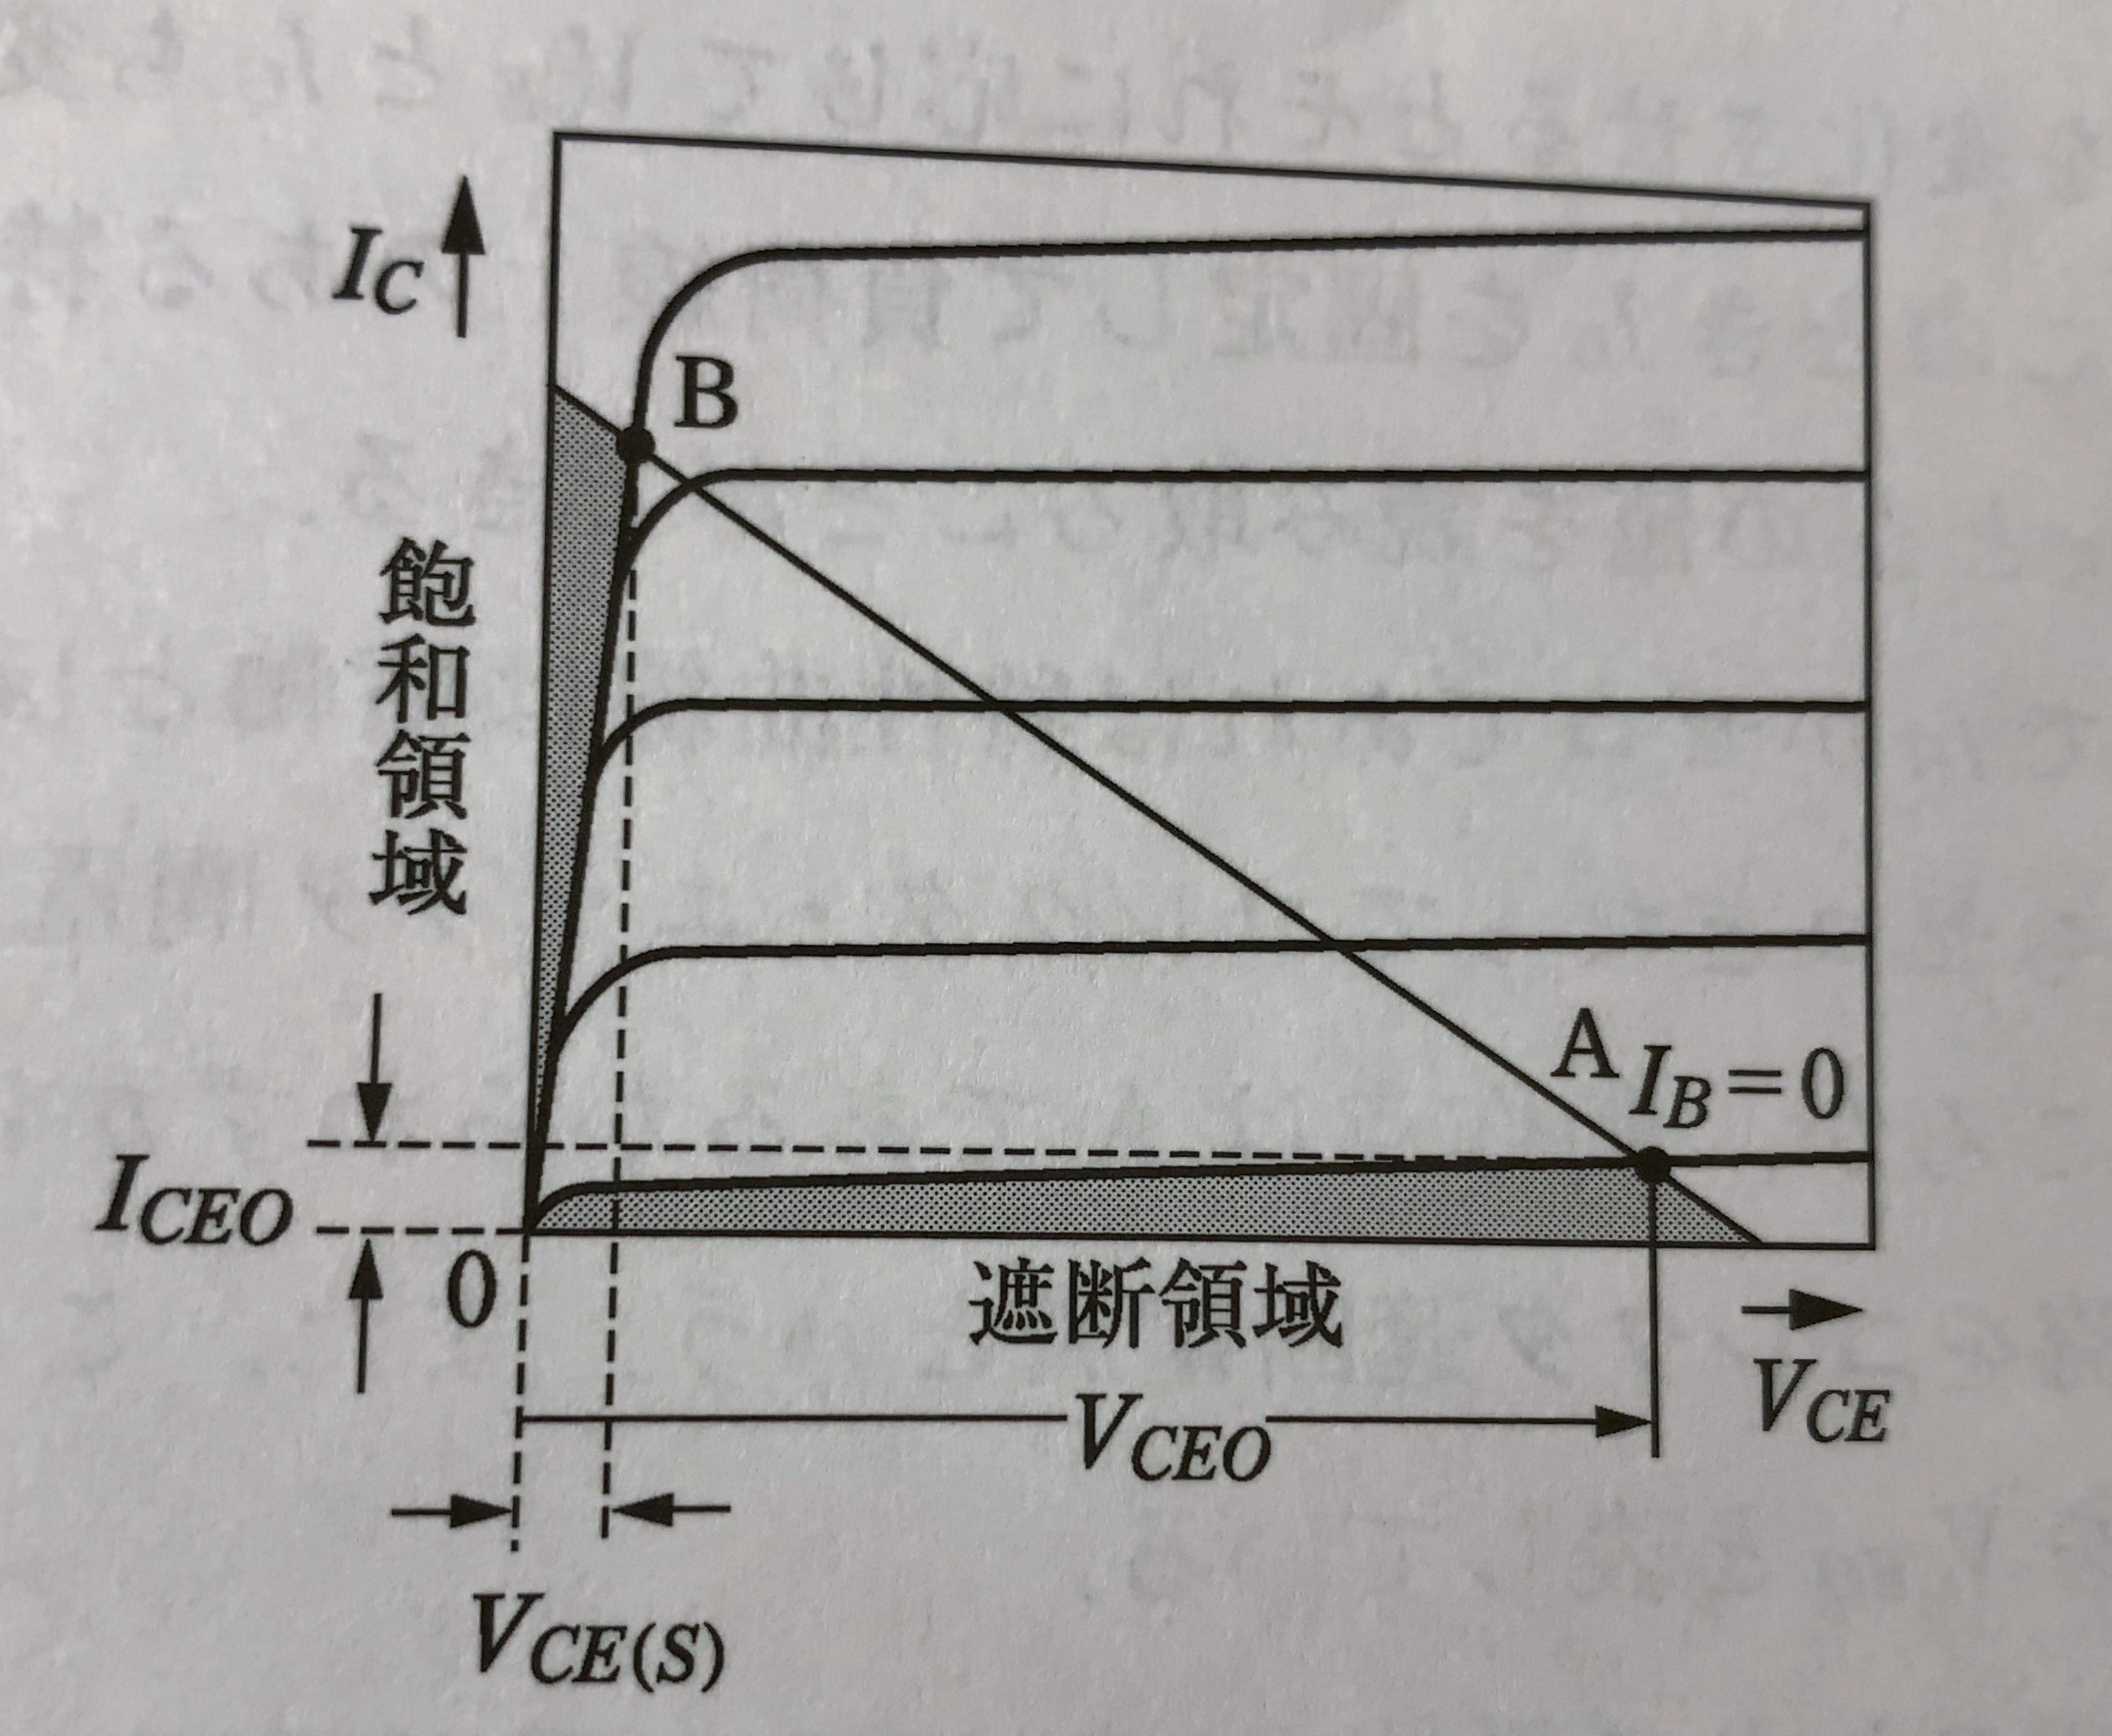
\includegraphics[bb=0 0 2589 2128,height=5cm]{parusu_9.jpg}
    \end{center}
    \caption{トランジスタの動作領域(参考文献7より)}
    \label{fig9}
\end{figure}

ここで、近似的に$I_{CEO} \fallingdotseq 0$、
$V_{CE(S)} \fallingdotseq 0$と考えると、トランジスタのスイッチング作用が分かる。
トランジスタのベース電流をゼロとしたとき、
コレクタ遮断電流$I_{CEO}$がごくわずか流れるが、この電流を無視すれば
動作は動作点は図\ref{fig10}に示す点$A$で、
トランジスタをスイッチに置き換えればOFF状態と考えることができ、
ベース電流を充分大きくするとコレクタ電流は飽和して、
コレクタ・エミッタの電圧$V_{CE(S)}$を無視すれば動作点は図\ref{fig11}の
$B$点で、トランジスタをスイッチに置き換えればON状態と考えられる。

\begin{figure}[h]
    \begin{center}
        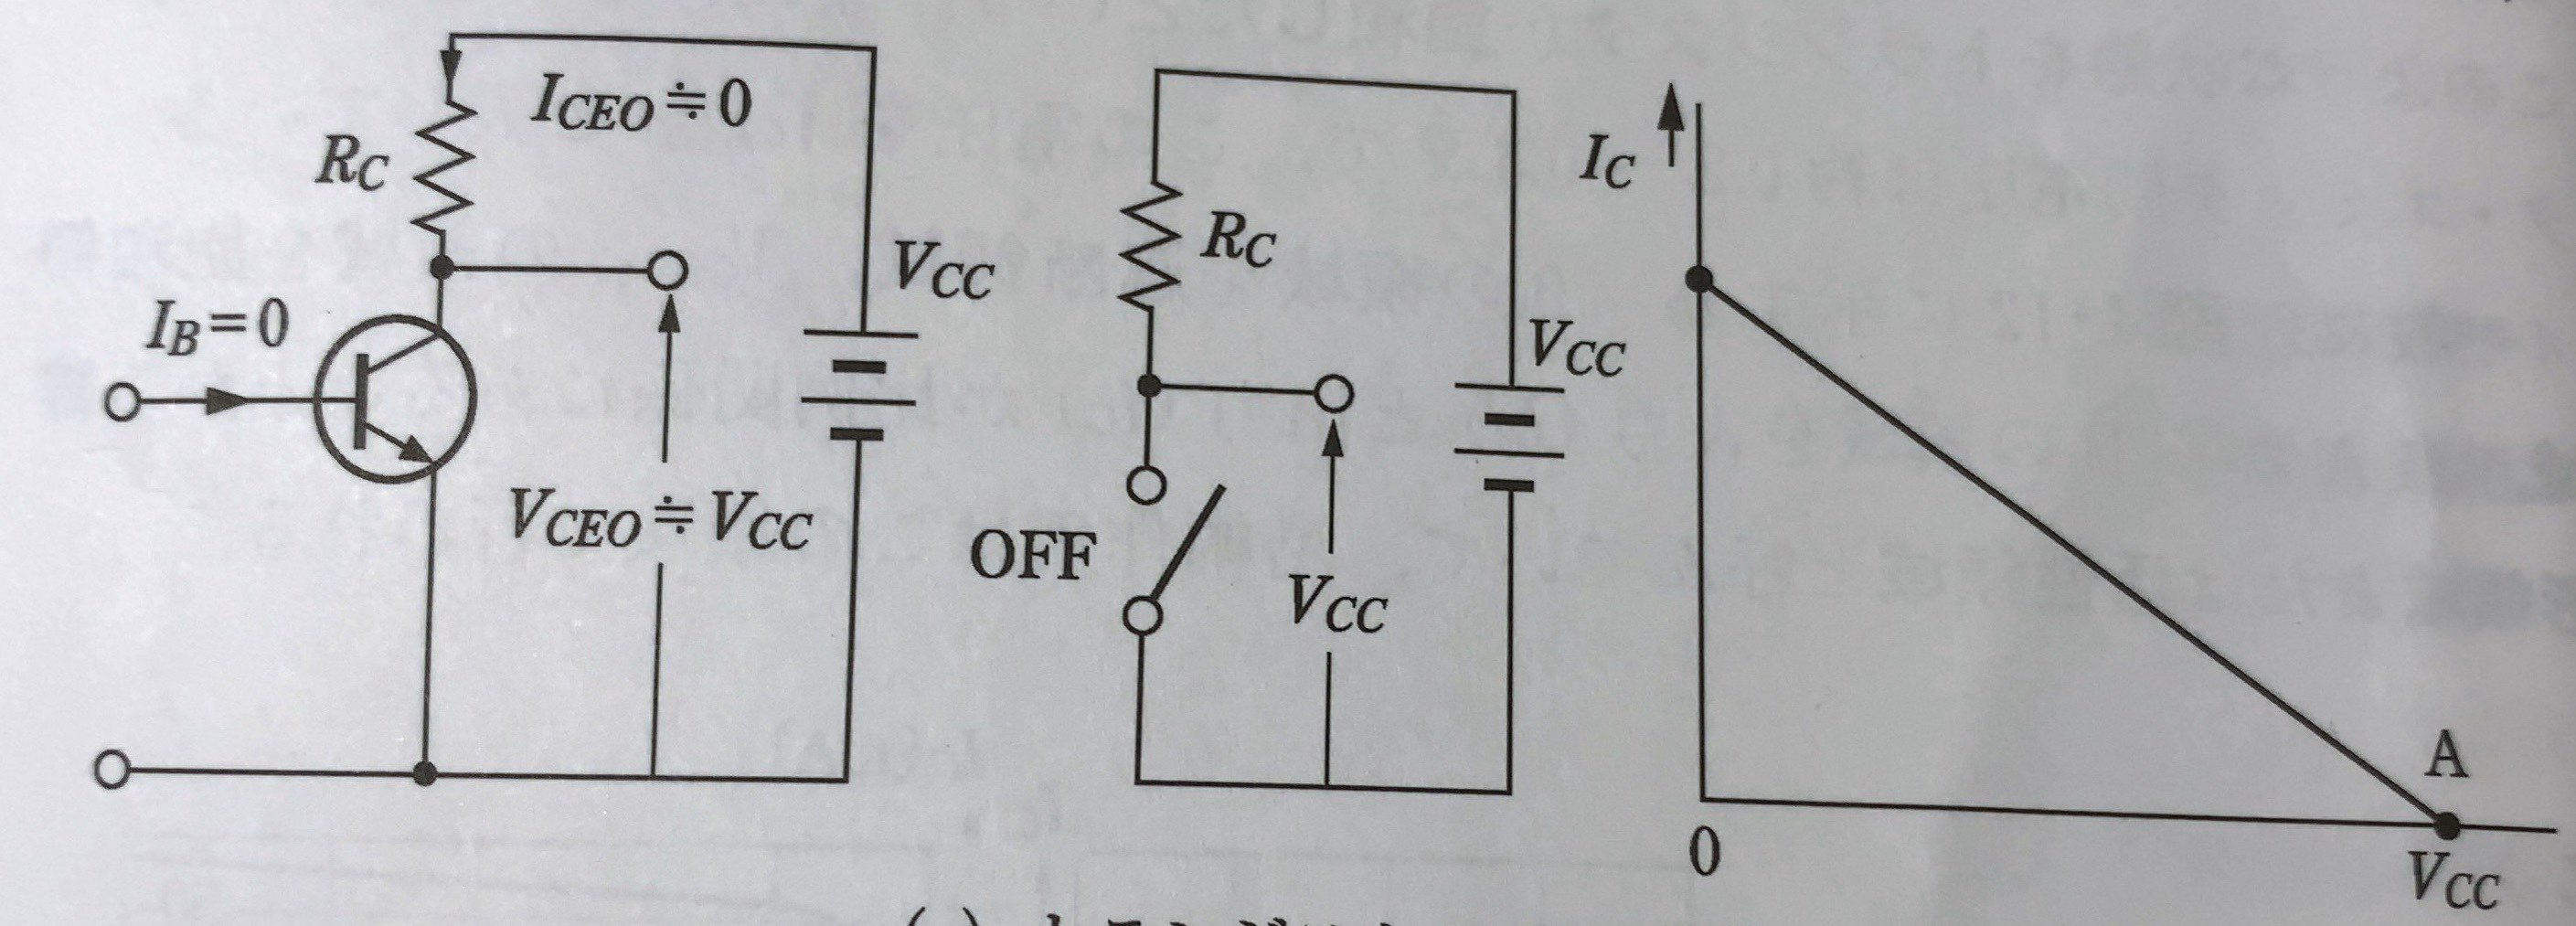
\includegraphics[bb=0 0 2818 1013,height=6cm]{parusu_10.jpg}
    \end{center}
    \caption{トランジスタのOFFの状態(参考文献7より)}
    \label{fig10}
\end{figure}
\begin{figure}[h]
    \begin{center}
        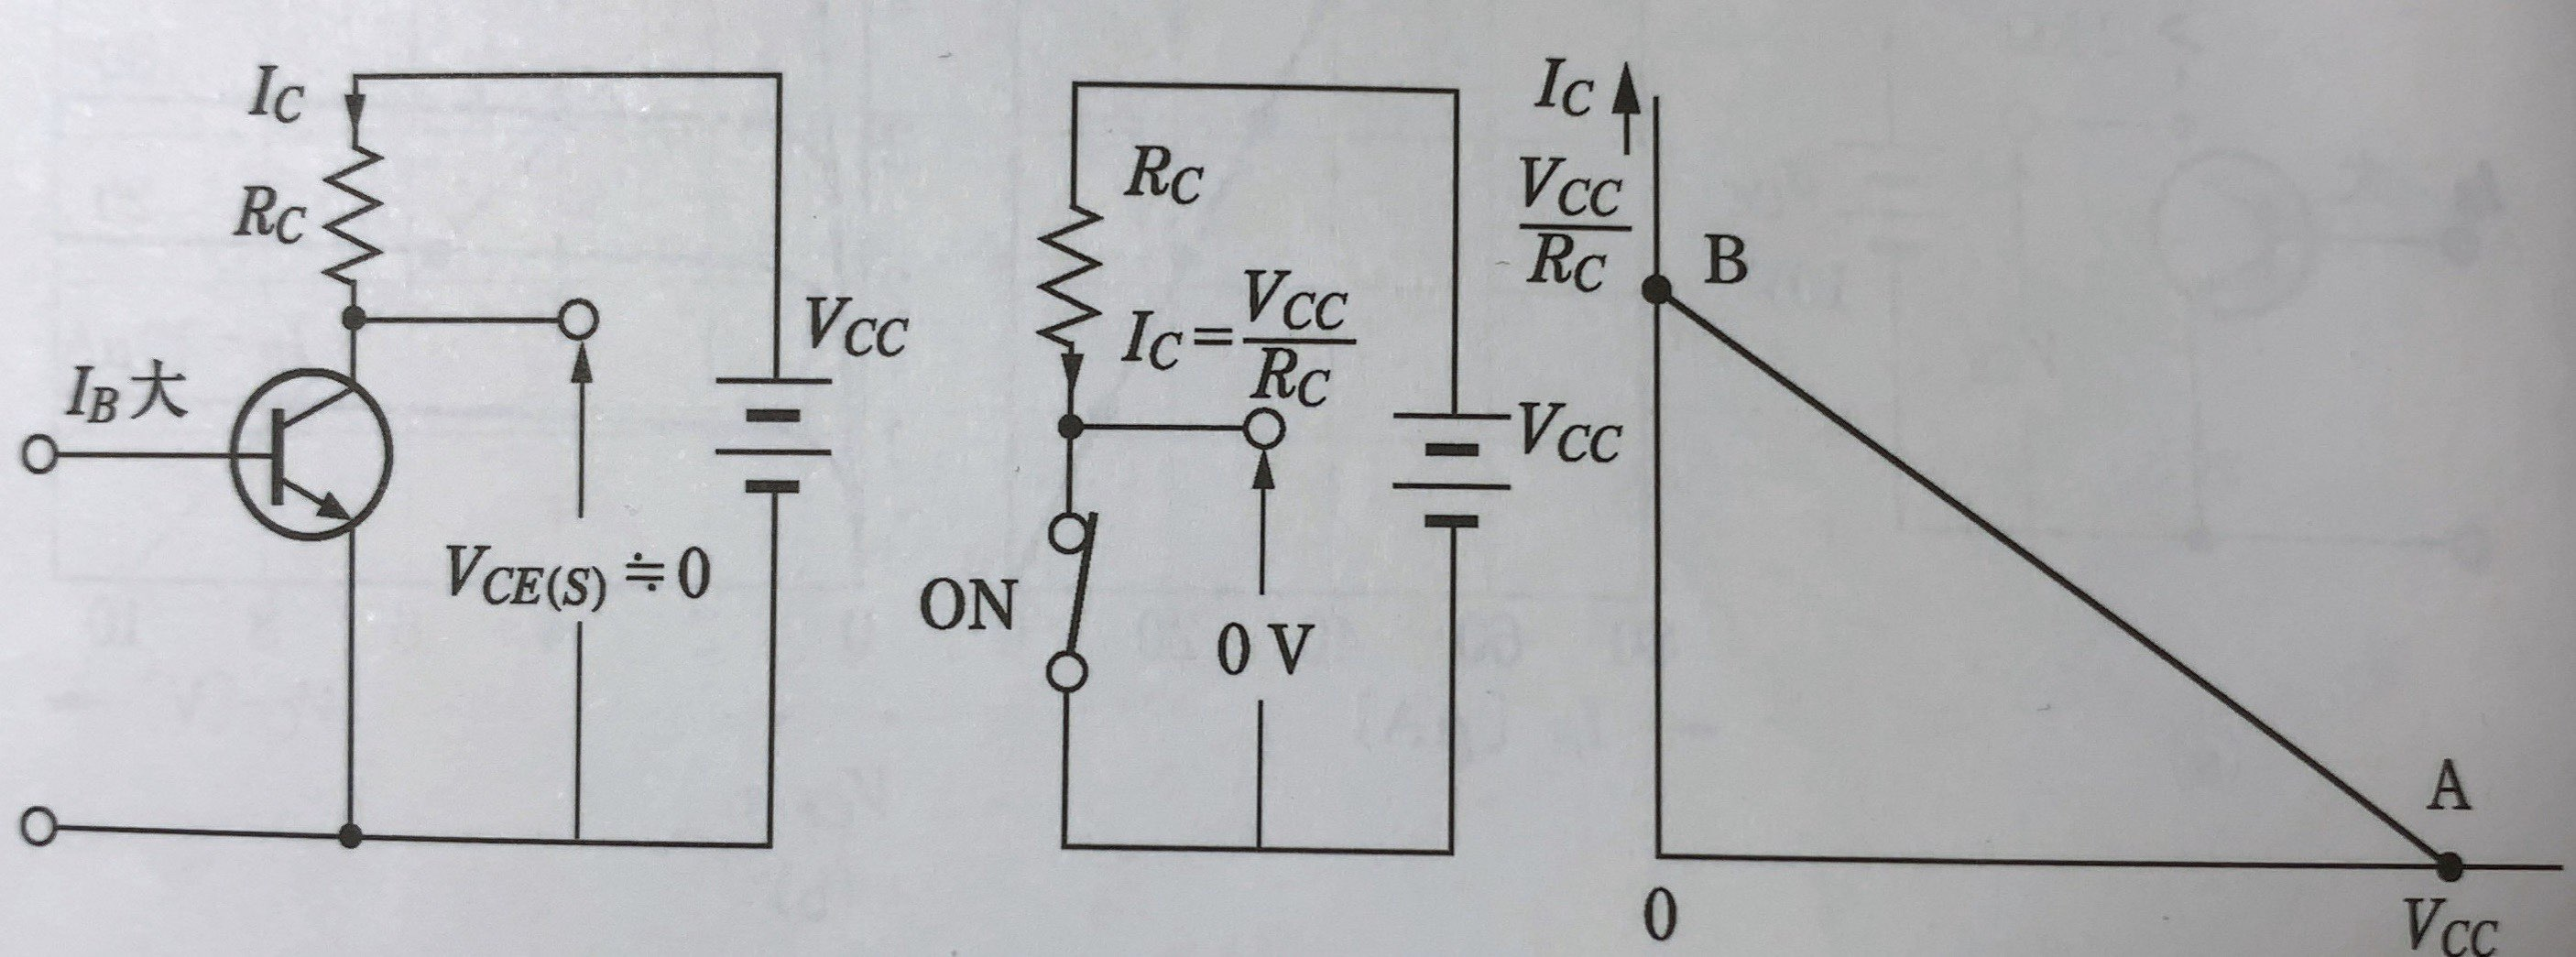
\includegraphics[bb=0 0 2812 1045,height=6cm]{parusu_11.jpg}
    \end{center}
    \caption{トランジスタのONの状態(参考文献7より)}
    \label{fig11}
\end{figure}

\clearpage
\subsection{レポート課題5}
\begin{shadebox}
    マルチバイブレータには本実験で扱ったものの他に単安定マルチバイブレータがある。
    これを含めた各マルチバイブレータの特徴および用途について述べよ。
\end{shadebox}
\subsubsection*{マルチバイブレータの特徴}
\begin{itemize}
    \item 無安定マルチバイブレータ
          \begin{itemize}
              \item 電源をいれると、連続してパルスを発生する。
              \item 2つの状態を常に行ったり来たりすることで発振する。
              \item その周波数は$R$と$C$の値によって決まる。$\frac{1}{CR}$に比例する。
          \end{itemize}
    \item 双安定マルチバイブレータ
          \begin{itemize}
              \item どちらの状態も安定している状態。
              \item 入力2発に対して出力1発が出る。
          \end{itemize}
    \item 単安定マルチバイブレータ
          \begin{itemize}
              \item 一方の状態は安定しているが、もう一方は安定しない状態。
              \item 入力パルスがあると、その波形に無関係に一定波形を出力する。
          \end{itemize}
\end{itemize}
\subsubsection*{マルチバイブレータの用途}
\begin{itemize}
    \item 無安定マルチバイブレータ
          \begin{itemize}
              \item 方形派パルスの発振器
              \item 自動車のウインカーの点滅
          \end{itemize}
    \item 双安定マルチバイブレータ
          \begin{itemize}
              \item 一定幅のパルスを作る
              \item チャタリング防止
          \end{itemize}
    \item 単安定マルチバイブレータ
          \begin{itemize}
              \item コンピュータの記憶回路
          \end{itemize}
\end{itemize}

\section{結論}
パルス回路の動作、原理、特性を動画とテキストにより理解し、パルス技術の基礎を学び、
スイッチング回路やマルチバイブレータの考察を通して、トランジスタについて詳しく知ることができた。

\clearpage
% 参考文献
\begin{thebibliography}{99}
    \label{sannkoubunnkenn_chapter}
    \bibitem[1]{rikadai}東京理科大学工学部情報工学科「情報工学実験1 2020年度」
    (2020/4/6)

    \bibitem[2]{cr_kairo}【CR回路】微分回路の波形・式・原理  |  西住工房

    \url{https://algorithm.joho.info/denki-denshi/cr-kairo-bibun-hakei-shiki-genri/#toc1}

    最終閲覧日:2020/6/23

    \bibitem[3]{condensa}スピードアップ・コンデンサの動作 | CQ出版社 オンライン・サポート・サイト CQ connect

    \url{https://cc.cqpub.co.jp/system/contents/2430/}

    最終閲覧日:2020/6/23

    \bibitem[4]{trunzista}トランジスタスイッチの高速化

    \url{http://www.purple.dti.ne.jp/masuki-sys/page133.html}

    最終閲覧日:2020/6/23

    \bibitem[5]{marutibaibure-ta}マルチバイブレータ回路の原理

    \url{https://hegtel.com/multivibrator-circuit.html}

    最終閲覧日:2020/6/23

    \bibitem[6]{suraido}マルチバイブレータ

    \url{https://www.slideshare.net/robotclub_kut/ss-33736293}

    最終閲覧日:2020/6/23

    \bibitem[7]{circuit}大類重範「ディジタル電子回路」
    日本理工出版会(2017/5/15)
\end{thebibliography}

\clearpage
\appendix
%%%%%%%%%%%%%%%%%%%%%%%%%%%%%%%%%%%%%%%%%%%%%%%%%%%%%%%
\end{document}
